% =========================================================================
%        LaTeX Template for PhD Thesis
% =========================================================================

%\RequirePackage[l2tabu, orthodox]{nag} % display more warnings

\documentclass{sokendai_thesis} % for final version
%\documentclass[todo]{sokendai_thesis} % print todo notes (generated by this command: \mytodo[inline]{this is just a todo note})


% =====================================================
%  User-defined Commands
% =====================================================

%\usepackage{amsmath}
%\usepackage[figure]{algorithm2e}
\usepackage{graphicx}
%\usepackage{mathtools}
%\usepackage{balance}
\usepackage{multirow}
\usepackage{comment}
%\usepackage{minted}
\usepackage{listings}
%\usepackage{enumitem}
%\usepackage{inconsolata}
\usepackage{courier}
\usepackage{subcaption}
%\usepackage[charter]{mathdesign}
% \def\rmdefault{bch} % not scaled
% \def\ttdefault{blg}
 
%\usepackage{amssymb}
\usepackage{pifont}
\newcommand{\cmark}{\ding{51}}%
\newcommand{\xmark}{\ding{55}}%
\definecolor{xgreen}{RGB}{44,160,44}

%\usepackage[hidelinks]{hyperref}

\lstdefinelanguage{pseudo}{
 morekeywords={for,if,then,else,send,to,ref,val,tag,val,true,false,inf,
   int,float,compute},
 %keywordstyle=\color{red},
 sensitive=false,
 morecomment=[l]{//},
}

\lstdefinelanguage{pregel}{
 morekeywords={for,in,do,until,fix,repeat,exists,forall,end,if,else,
  let,true,false,fst,snd,to_int,to_float,ref,val,inf,local,remote,V,
  input,output,field,extern,maximum,minimum,sum,and,or,random,
  Nbr,In,Out,Id,int,float,bool,this},
 %keywordstyle=\color{red},
 sensitive=true,
 morecomment=[l]{//},
}
\lstset{
 basicstyle=\small\ttfamily,
 commentstyle=\small\color{xgreen}\ttfamily,
 language=pregel,
 numbers=left,
 xleftmargin=0.05\textwidth,
 stepnumber=1,
 numberfirstline=false
}

\newcommand{\plus}{\raisebox{.25ex}{\scalebox{.8}{+}}}
\newcommand{\plusplus}{\plus\plus}
%\SetKwInput{KwInput}{Input}
%\SetKwInput{KwOutput}{Output}
\makeatletter
\newcommand{\shorteq}{%
  \settowidth{\@tempdima}{--}%
  \resizebox{\@tempdima}{\height}{=}%
}
\makeatother
\newcommand{\shorteqq}{\mathop{\shorteq\shorteq}}
\newcommand{\knows}[2]{\mathrm K_{#1}\,{#2}}
%\def\ttdefault{txtt}

\newcommand{\hsp}[1]{\hspace{-3em}\hbox{#1}}

% =====================================================
%  Thesis Info
% =====================================================

\title{Towards Intuitive and Efficient Vertex-Centric Graph Processing}
\author{Yongzhe Zhang}
\date{June 2017}
\crest{Crest/sokendai_crest.pdf} % comment out if you don't have a crest.
%\keywords{Latex Template, Sokendai, PhD Thesis} % for PDF meta-info


% =====================================================
%  Others
% =====================================================

% Typeset only specified chapters
%\includeonly{Manuscript/Introduction/introduction}


% =====================================================
%  Front Matter
% =====================================================

\begin{document}

\frontmatter
\maketitle

\listoftodos

\chapter*{Abstract}

Pregel is a popular parallel computing model for dealing with large-scale graphs.
However, it can be tricky to implement graph algorithms correctly and efficiently in Pregel's vertex-centric model, especially when the algorithm has multiple computation stages, complicated data dependencies, or even communication over dynamic internal data structures.
Some domain-specific languages (DSLs) have been proposed to provide more intuitive ways to implement graph algorithms, but due to the lack of support for \emph{remote access} --- reading or writing attributes of other vertices through references --- they cannot handle the above mentioned dynamic communication, causing a class of Pregel algorithms with fast convergence impossible to implement.

To address this problem, we design and implement Palgol, a more declarative and powerful DSL which supports remote access.
In particular, programmers can use a more declarative syntax called \emph{chain access} to naturally specify dynamic communication as if directly reading data on arbitrary remote vertices.
By analyzing the logic patterns of chain access, we provide a novel algorithm for compiling Palgol programs to efficient Pregel code.
Furthermore, we recognize the limitation of Pregel's message passing interface in handling graph algorithms with multiple communication channels, so we extend the Pregel framework with the \emph{message channel interface}, to enable more optimizations for message reduction.
We demonstrate the power of Palgol by using it to implement a bunch of practical Pregel algorithms and compare them with hand-written code.
The evaluation result shows that the efficiency of Palgol is comparable with that of hand-written code. %, and our extended Pregel framework can further improve the performance.
As a future work, we are going to compile Palgol to our new Pregel interface to achieve better performance.

\tableofcontents
%\listoffigures
%\listoftables
%% List of algorithms
%\listofalgorithms \addcontentsline{toc}{chapter}{List of Algorithms}

% =====================================================
%  Main Matter
% =====================================================

\mainmatter

\chapter{Introduction}

The rapid increase of graph data in real world calls for efficient analysis on massive graphs.
However, graph computation is in general difficult to parallelize or scale, due to the inherent interdependencies in graph data.
In this work, we focus on a particular type of graph processing system that adopts the "Think like a vertex" paradigm, and indentify the difficulties in programming and optimization.
We therefore design a domain-specific language to provide a high-level abstraction and customize a graph processing system for message reduction, trying to give an intuitive and efficient solution for this problem.

\section{Pregel: Graph Processing in Vertex-Centric Paradigm}

Google's Pregel~\cite{pregel} is one of the most popular framework for processing large-scale graphs, which is based on the bulk-synchronous parallel (BSP) model~\cite{bsp}.
It adopts the \emph{vertex-centric} computing paradigm to achieve high parallelism and scalability.
In Pregel, the input is in general a directed graph, and each vertex is associated with a mutable user-defined state.
Following the Bulk-Synchronous Parallel (BSP) model~\cite{bsp}, computation is split into \emph{supersteps} mediated by \emph{message passing.}
Within each superstep, all the vertices execute the same user-defined function in parallel, and each vertex can read the messages sent to it in the previous superstep, modify its own state, and send messages to other vertices.
Global barrier synchronization happens at the end of each superstep, delivering messages to their designated receivers before the next superstep.
In general, a vertex can send any number of messages to any other vertices, but there is no guaranteed order among the messages.
%Also, in Pregel, only a single message type is allowed, so programmers should encode different types in one if they need to pass multiple types of messages.
A vertex is active at the beginning of execution, and can deactivate itself by ``voting to halt.''
When inactive, it can only be activated by receiving messages.
(\autoref{fig:voteToHalt} illustrates this mechanism with a state transition diagram.)
Computation terminates when all vertices become inactive. %in a particular superstep.
\begin{figure}[ht]
 \centering
 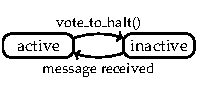
\includegraphics[width=0.35\textwidth]{figures/active.pdf}
 \caption{Vertex State Machine}
 \label{fig:voteToHalt}
\end{figure}

Besides vertex-to-vertex message passing, Pregel provides \emph{aggregators}, a mechanism for global communication.
Every vertex can provide a value to an aggregator in a superstep; the system then combines these values by a reduction operator and makes the result available at the beginning of the next superstep.
Pregel has a bunch of predefined aggregators for various types, like $\mathit{max}$ and $\mathit{min}$ for numeric values, but programmers may also define their own aggregators by providing a reduction operator and an appropriate default value.
Whether built-in or user-defined, an aggregation operator should be commutative and associative \todo{define this as ``accumulative''?}, with the default value being an identity.
Being simple, Pregel has demonstrated its usefulness in implementing many interesting graph algorithms \cite{pregel,QuWH12,connectivity,optimizing,XiYZ14}.

\section{Problem in Existing Pregel Frameworks}

Despite the power of Pregel, it is a big challenge to implement a graph algorithm correctly and efficiently in it \cite{connectivity}, especially when the algorithm consists of multiple stages and complicated data dependencies.
For such algorithms, programmers need to write an exceedingly complicated \textit{compute()} function as the loop body, which encodes all the stages of the algorithm. %, each being one or more supersteps interrelated by message passing.
Message passing makes the code even harder to maintain, because one has to trace where the messages are from and what information they carry in each superstep.
Some attempts have been made to ease Pregel programming by proposing domain-specific languages (DSLs), such as Green-Marl~\cite{green14} and Fregel~\cite{fregel}.
These DSLs allow programmers to write a program in a compositional way to avoid writing a complicated loop body, and provide neighboring data access to avoid explicit message passing.
Furthermore, programs written in these DSLs can be automatically translated to Pregel by fusing the components in the programs into a single loop, and mapping neighboring data access into message passing.
However, for efficient implementation, the existing DSLs impose a severe restriction on data access --- each vertex can only access data on their neighboring vertices.
In other words, they do not support general \emph{remote data access} --- reading or writing attributes of other vertices through references.

\begin{comment}
In addition to the difficulties in mapping the graph algorithms to Pregel, the Pregel's interface is unsuitable for implementing the algorithms containing various stages or requiring data communication for different purposes, and may potentially decrease the performance.
This is due to the single message type throughout the whole computation, and the complex side effects of vertex-inactivation interface:
\begin{itemize}\setlength\itemsep{0em}
\item
 \textit{Single message type}.
 In Pregel, programmers need to specify a message type in advance, and the implement the \emph{compute()} function that handles or emits the messages in this type only.
 However, some graph algorithms actually need different message types for different purposes, in which case it may consume more space and bring the overhead of data encoding/decoding.
\item
 \textit{Side effects in vertex-inactivation}.
 Many graph algorithms can be optimized by the vertex-inactivation interface, for example to skip the vertices that are already converged.
 However, the vertex state is also used to control the termination, and affects the computation of aggregator, which makes it not always applicable in graph algorithms.
\end{itemize}
\end{comment}

Remote data access is, however, important for describing a class of Pregel algorithms that aim to accelerate information propagation (which is a crucial issue in handling graphs with large diameters~\cite{connectivity}) by maintaining a dynamic internal structure for communication.
For instance, a parallel pointer jumping algorithm maintains a tree (or list) structure in a distributed manner by letting each vertex store a reference to its current parent (or predecessor), and during the computation, every vertex constantly exchanges data with the current parent (or predecessor) and modifies the reference to reach the root vertex (or the head of the list).
Such computational patterns can be found in the algorithms like the Shiloach-Vishkin connected component algorithm~\cite{connectivity} (see \autoref{sec:sv-algorithm} for more details), the list ranking algorithm (see \autoref{sec:list-ranking}) and Chung and Condon's minimum spanning forest (MSF) algorithm~\cite{boruvka}.
However, these computational patterns cannot be implemented with only neighboring access, and therefore cannot be expressed in any of the existing high-level DSLs.

It is, in fact, hard to equip DSLs with efficient remote reading.
First, when translated into Pregel's message passing model, remote reads require multiple rounds of communication to exchange information between the reading vertex and the remote vertex, and it is not obvious how the communication cost can be minimized.
Second, remote reads would introduce more involved data dependencies, making it difficult to fuse program components into a single loop.
Things become more complicated when there is \emph{chain access}, where a remote vertex is reached by following a series of references.
Furthermore, it is even harder to equip DSLs with remote writes in addition to remote reads.
For example, Green-Marl detects read/write conflicts, which complicate its programming model; Fregel has a simpler functional model, which, however, cannot support remote writing without major extension.
A more careful design is required to make remote reads and writes efficient and friendly to programmers.

\section{Contribution of My Research}

In this work, we propose a more powerful DSL called Palgol (for {\bf P}regel {\bf algo}rithmic {\bf l}anguage) that supports remote data access.
%In particular, programmers are allowed to use a more declarative syntax called
%\emph{global field access}, to directly read data on remote vertices.
By structuring supersteps in a high-level vertex-centric computation model and analyzing the logic patterns of global field access, we provide a novel algorithm for compiling Palgol programs to efficient Pregel code. 
The main contributions are as follows:
\begin{itemize}\setlength\itemsep{0em}
 \item
  We propose a new high-level model for vertex-centric computation, where the concept of \emph{algorithmic supersteps} is introduced as the basic computation unit for constructing vertex-centric computation in such a way that remote reads and writes are ordered in a safe way.
  %Using algorithmic supersteps along with \emph{sequence} and \emph{iteration}, graph algorithms can be expressed clearly and concisely.

 \item
  Based on the new model, we design and implement Palgol, a more declarative and powerful DSL, which supports both remote reads and writes, and allows programmers to use a more declarative syntax called \emph{chain access} to directly read data on remote vertices.
  For efficient compilation from Palgol to Pregel, we develop a logic system to compile chain access to efficient message passing where the number of supersteps is reduced whenever possible. %without redundant communications, and an algorithm to translate Palgol programs to Pregel programs where the number of supersteps is reduced whenever possible. 

 \item
  We demonstrate the power of Palgol by working on a set of representative examples, including the Shiloach-Vishkin connected component algorithm and the list ranking algorithm, which use communication over dynamic data structures to achieve fast convergence.

 \item
  Based on the Palgol's high-level model, we further study the efficient implementation of graph algorithms in distributed environment.
  We propose an extension of Pregel framework with message channel interfaces, which allows programmers to use different message types and separately manage or optimize each communication channel, to reduce the message size in computation.

 \item
  The result of our evaluation is encouraging.
  The efficiency of Palgol is comparable with hand-written code for many representative graph algorithms on practical big graphs, where execution time varies from a $2.53\%$ speedup to a $6.42\%$ slowdown in ordinary cases, while the worst case is less than a $30\%$ slowdown.

\end{itemize}

\section{Outline}

We introduce the Palgol language in \autoref{sec:palgol-lang}, and in \autoref{sec:compilation}, we show how to compile Palgol programs to the state transition machine (STM) --- a typical intermediate representation of Palgol programs.
\autoref{sec:custom} describes our custom Pregel framework as a new backend of Palgol, and \autoref{sec:evaluation} presents the evaluation results.
\autoref{sec:conclusions} concludes this dissertation progress report.

\chapter{The Palgol Language}
\label{sec:palgol-lang}

This chapter first introduces a high-level vertex-centric programming model~(\autoref{sec:palgol-model}), in which an algorithm is decomposed into atomic vertex-centric computations and high-level combinators, and a vertex can access the entire graph through the references it stores locally.
Next we define the Palgol language based on this model, and explain its syntax and semantics~(\autoref{sec:syntax}).
Then we use three representative examples (in \autoref{sec:taste}) --- the single-source shortest path algorithm, the Shiloach-Vishkin connected component algorithm and the list ranking algorithm --- to demonstrate how Palgol can concisely describe vertex-centric algorithms, and how dynamic internal structures are maintained using remote access.
Finally, we discuss a useful feature of Palgol that help programmers easily deactivate vertices during the computation.

%In this section, we present our high-level DSL Palgol to describe vertex-centric graph algorithms with flexible remote access.
%We start from introducing a high-level model, in which an algorithm description has a more direct correspondence with the Pregel model.
%Then we define the Palgol language based on this model, and explain its syntax and semantics.
%Finally we use two examples to demonstrate how Palgol can concisely describe some Pregel algorithms using remote access.

\section{The High-Level Model}
\label{sec:palgol-model}

The high-level model we propose uses remote reads and writes instead of message passing to allow programmers to describe vertex-centric computation more intuitively. %, making it more suitable for describing an algorithm.
Moreover, the model remains close to the Pregel computation model, in particular keeping the vertex-centric paradigm and barrier synchronization, making it possible to automatically derive a valid and efficient Pregel implementation from an algorithm description in this model, and in particular arrange remote reads and writes without data conflicts.

In our high-level model, the computation is constructed from some basic components which we call \emph{algorithmic supersteps}.
An algorithmic superstep is a piece of vertex-centric computation which takes a graph containing a set of vertices with local states as input, and outputs the same set of vertices with new states.
Using algorithmic supersteps as basic building blocks, two high-level operations \emph{sequence} and \emph{iteration} can be used to glue them together to describe more complex vertex-centric algorithms that are iterative and/or consist of multiple computation stages:
the \emph{sequence} operation concatenates two algorithmic supersteps by taking the result of the first step as the input of the second one, and the \emph{iteration} operation repeats a piece of vertex-centric computation until some termination condition is satisfied.
%Compared with the Pregel model, where supersteps operate on not only vertex states but also messages, our model . \todo{focus on graph transformations} %, since each algorithmic superstep independently describes a piece of computation, making people easier to reason about different computation stages separately.
%A particular advantage of the compositional approach is that, it naturally uses the barrier synchronization, which is consistent with the Pregel model.

The distinguishing feature of algorithmic supersteps is remote access.
Within each algorithmic superstep (illustrated in \autoref{fig:algostep}), all vertices compute in parallel, performing the same computation specified by programmers.
A vertex can read the fields of any vertex in the input graph; it can also write to arbitrary vertices to modify their fields, but the writes are performed on a separate graph rather than the input graph (so there are no read-write conflicts).
We further distinguish \emph{local writes} and \emph{remote writes} in our model:
local writes can only modify the current vertex's state, and are first performed on an intermediate graph (which is initially a copy of the input graph);
next, remote writes are propagated to the destination vertices to further modify their intermediate states.
Here, a remote write consists of a remote field, a value and an ``accumulative'' assignment (like \texttt{+=} and \texttt{|=}), and that field of the destination vertex is modified by executing the assignment with the value on its right-hand side.
We choose to support only accumulative assignments so that the order of performing remote writes does not matter.

\begin{figure}[t]
 \centering
 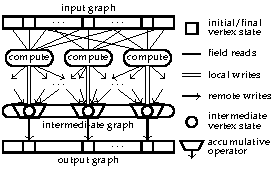
\includegraphics[width=0.75\textwidth]{figures/model.pdf}
 \caption{In an algorithmic superstep, every vertex performs local computation (including field reads and local writes) and remote updating in order.}
 \label{fig:algostep}
 \vspace{-2.5ex}
\end{figure}

The distinguishing feature of algorithmic supersteps is remote access.
Within each algorithmic superstep (illustrated in \autoref{fig:algostep}), all vertices compute in parallel, performing the same computation specified by programmers.
A vertex can read the fields of any vertex in the input graph; it can also write to arbitrary vertices to modify their fields, but the writes are performed on a separate graph rather than the input graph, to completely avoid read-write conflicts.
We further distinguish \emph{local writes} and \emph{remote writes} in our model:
local writes can only modify the current vertex's state, and are first performed on an intermediate graph (which is initially a copy of the input graph);
next, remote writes are propagated to the destination vertices to further modify their intermediate states.
Here, a remote write consists of a remote field, a value and an ``accumulative'' assignment (like \texttt{+=} and \texttt{|=}), and that field of the destination vertex is modified by executing the assignment with the value on its right-hand side.
We choose to support only accumulative assignments so that the order of performing remote writes does not matter.

More precisely, an algorithmic superstep is divided into the following two phases:
\begin{itemize}\setlength\itemsep{0em}
 \item a \emph{local computation} (LC) phase, in which a copy of the input graph is created as the intermediate graph, and then each vertex can read the state of any vertex in the input graph, perform local computation, and modify its own state in the intermediate graph, and
 \item a \emph{remote updating} (RU) phase, in which each vertex can modify the states of any vertices in the intermediate graph by sending remote writes.
 After all remote writes are processed, the intermediate graph is returned as the output graph.
\end{itemize}
Among these two phases, the RU phase is optional, in which case the intermediate graph produced by the LC phase is used directly as the final result.

\section{An Overview of Palgol}
\label{sec:syntax}

We present our DSL Palgol next, whose design follows the high-level model we introduced in the previous subsection.
Figure~\ref{fig:syntax-simplified} shows the essential part of the syntax of Palgol.
%(A few more constructs will be introduced in Section~\ref{sec:advanced}.)
As described by the syntactic category \textit{step}, an algorithmic superstep in Palgol is a code block
enclosed by ``\textbf{for} \textit{var} \textbf{in} \textbf{V}'' and ``\textbf{end}'', where \textit{var} is a variable name that can be used in the code block for referring to the current vertex.
Such steps can then be composed (by sequencing) or iterated until a termination condition is met (by enclosing them in ``\textbf{do}'' and ``\textbf{until} \ldots'').
Palgol supports several kinds of termination conditions, but in this report we focus on only one kind of termination condition called \textit{fixed point}, since it is extensively used in many algorithms.
The semantics of fixed-point iteration is iteratively running the program enclosed by \textbf{do} and \textbf{until}, until the specified fields stabilize.
%\todo{perhaps mention there are others}

\begin{figure}[t]
\normalsize
\[
\begin{array}{lclr}
%\mathit{int} & = & \hbox{integer} \\
%\mathit{float} & = & \hbox{floating-point number} \\
%\mathit{var} & = & \hbox{identifier starting with lowercase letter} \\
%\mathit{field} & = & \hbox{identifier starting with capital letter} \\
%\\
\mathit{prog}  & \Coloneqq & \mathit{step}~|~\mathit{prog_1}\ldots\mathit{prog_n}~|~\mathit{iter} \\
\mathit{iter} & \Coloneqq & \mathbf{do}~\langle~\mathit{prog}~\rangle~\mathbf{until}~\mathbf{fix}~[~\mathit{field_1},\ldots,\mathit{field_n}~] \\
\mathit{step}& \Coloneqq & \mathbf{for}~\mathit{var}~\mathbf{in}~\mathbf{V}~\langle~\mathit{block}~\rangle~\mathbf{end} \\
\mathit{block} & \Coloneqq & \mathit{stmt_1} \ldots \mathit{stmt_n} \\
\mathit{stmt}  & \Coloneqq & \mathbf{if}~\mathit{exp}~\langle~\mathit{block}~\rangle~|~\mathbf{if}~\mathit{exp}~\langle~\mathit{block}~\rangle~\mathbf{else}~\langle~\mathit{block}~\rangle \\
 & | & \mathbf{for}~(\mathit{var}\leftarrow\mathit{exp})~\langle~\mathit{block}~\rangle \\
 & | & \mathbf{let}~\mathit{var}=\mathit{exp} \\
 & | & \mathbf{local}\mathit{_{opt}}~\mathit{field}~[~\mathit{var}~]~\mathit{op_{local}}~\mathit{exp} & \hsp{-- local write} \\
 & | & \mathbf{remote}~\mathit{field}~[~\mathit{exp}~]~\mathit{op_{remote}}~\mathit{exp} & \hsp{-- remote write} \\
\mathit{exp}   & \Coloneqq & \mathit{int}~|~\mathit{float}~|~\mathit{var}~|~\mathbf{true}~|~\mathbf{false}~|~\mathbf{inf} \\
 & | & \mathbf{fst}~\mathit{exp}~|~\mathbf{snd}~\mathit{exp}~|~(\mathit{exp},\mathit{exp}) \\
 & | & \mathit{exp}.\mathbf{ref}~|~\mathit{exp}.\mathbf{val}~|~\{\mathit{exp},\mathit{exp}\}~|~\{\mathit{exp}\} & \hsp{-- specialized pair} \\
 & | & \mathit{exp}~?~\mathit{exp}:\mathit{exp}~|~(~\mathit{exp}~)~|~\mathit{exp}~\mathit{op_{binary}}~\mathit{exp}~|~\mathit{op_{unary}}~\mathit{exp} \\
 & | & \mathit{field}~[~\mathit{exp}~] & \hsp{-- global field access} \\
 & | & \mathit{func_{opt}}~[~\mathit{exp}~|~\mathit{var}\leftarrow\mathit{exp},\mathit{exp_1},\ldots,\mathit{exp_n}~] \\
\mathit{func}  & \Coloneqq & \mathbf{maximum}~|~\mathbf{minimum}~|~\mathbf{sum}~|~\ldots \\
 \end{array}
\]
\caption{Essential part of Palgol syntax. Palgol is indentation-based, and two special tokens `$\langle$' and `$\rangle$' are introduced to represent the change of indentation level.}
\label{fig:syntax-simplified}
\vspace{-2ex}
\end{figure}

Corresponding to an algorithmic superstep's remote access capabilities, in Palgol we can read a field of an arbitrary vertex using a global field access expression of the form $\mathit{field}~[\,\mathit{exp}\,]$, 
where $\mathit{field}$ is a user-specified field name and $\mathit{exp}$ should evaluate to a vertex id.
Such expression can be updated by local or remote assignments, where an assignment to a remote vertex should always be accumulative and prefixed with the keyword $\mathbf{remote}$.
%and use accumulative assignment operation only.
One more thing about remote assignments is that they take effect only in the RU phase (after the LC phase), regardless of where they occur in the program.
%Such syntax looks similar to an array access, and indeed, one can regard a field as a global array, so that when a vertex id is given, the value of the field on that vertex is returned.
%In Palgol, we can also update a remote field using an accumulative assignment statement prefixed with the keyword $\mathbf{remote}$.
%Remote updating statements take effect only in the RU phase (after the LC phase), regardless of where they occur in the program, and the assignment operation can only be accumulative.
%To better distinguish the two kinds of updating statements, local updating statements are prefixed with the \textbf{local} keyword.
%\end{itemize}

There are some predefined fields that have special meaning in our language.
%$\mathbf{Nbr}$, $\mathbf{In}$, $\mathbf{Out}$ are by default the edge lists, where 
$\mathbf{Nbr}$ is the edge list in undirected graphs, and $\mathbf{In}$ and $\mathbf{Out}$ respectively store incoming and outgoing edges for directed graphs.
Essentially, these are normal fields of a predefined type for representing edges, and most importantly, the compiler assumes a form of symmetry on these fields (namely that every edge is stored consistently on both of its end vertices), and uses the symmetry to produce more efficient code.
%Then, $\mathbf{Id}$ is an immutable field that stores the vertex identifier for each vertex (required by the Pregel framework), whose type is user-specified but currently we can simply treat it as an integer.

The rest of the syntax for Palgol steps is similar to an ordinary programming language.
Particularly, we introduce a specialized pair type (expressions in the form of $\{\mathit{exp},\mathit{exp}\}$) for representing a reference with its corresponding value (e.g., an edge in a graph), and use $.\mathbf{ref}$ and $.\mathbf{val}$ respectively to access the reference and the value respectively, to make the code easy to read.
Some functional programming constructs are also used here, like let-binding and list comprehension.
There is also a foreign function interface that allows programmers to invoke functions written in a general-purpose language, but we omit the detail from the thesis.

\section{A Taste of Palgol}
\label{sec:taste}

In this section, we use three examples to demonstrate how to describe vertex-centric algorithms in Palgol.
First, we discuss a typical algorithm called the single-source shortest path (SSSP), then two more interesting examples called the Shiloach-Vishkin (S-V) Algorithm and the list ranking algorithm are introduce, which shows more important features of Palgol.

\subsection{Single-Source Shortest Path Algorithm}
\label{sec:sssp}

The single-source shortest path problem is among the best known in graph theory and arises in a wide variety of applications.
To understand this algorithm, we first have a look at how it is implemented in Google's Pregel system~\cite{pregel} in Figure~\ref{fig:sssp-pregel}.
\begin{figure}[thp]
\vspace{-2ex}
\begin{lstlisting}[basicstyle=\small\ttfamily,numbers=none,language=c++]
class ShortestPathVertex : public Vertex<int, int, int> {
   void Compute(MessageIterator* msgs) {
      int minDist = vertex_id() == 0 ? 0 : INF;
      for (; !msgs->Done(); msgs->Next())
         minDist = min(minDist, msgs->Value());
      if (minDist < GetValue()) {
         *MutableValue() = minDist;
         OutEdgeIterator iter = GetOutEdgeIterator();
         for (; !iter.Done(); iter.Next())
            SendMessageTo(iter.Target(),
               minDist + iter.GetValue());
      }
      VoteToHalt();
   }
};
\end{lstlisting}
\vspace{-2ex}
\caption{Google's SSSP Pregel program~\protect\cite{pregel}}
\label{fig:sssp-pregel}
\end{figure}

This program assumes that the initial distance associated with each vertex is infinite (INF).
In each superstep, every vertex first receives messages containing the potentially minimum distances from the source computed by its neighbors, and chooses the smallest one among them.
If that distance is smaller than the one it currently stores, then it updates its own distance, and sends messages to inform all its neighbors of their potentially minimum distances from its perspective.
%, activating the neighboring vertices in the next superstep.
Every node votes to halt at the end, and in the next superstep only those nodes who have received messages will be activated.
The computation is performed iteratively until all vertices become inactive.

Despite the obscure Pregel implementation, which is cluttered with language-specific and low-level details (in particular message passing), the idea of this algorithm is fairly simple, which is an iterative computation until the following equation holds:
$$ \mathit{dist}[v] =\begin{cases}0 & \text{$v$~is the source} \\ \min_{u\in \mathit{In}(v)}~(\mathit{dist}[u]~+~\mathit{len}(v,~u)) & \text{otherwise} \end{cases} $$
We can concisely capture the essence of the shortest path algorithm in a Palgol program, as shown in Figure~\ref{fig:sssp-palgol}.
In this program, we store the distance of each vertex from the source in the $D$~field, and use a boolean field~$A$ to indicate whether the vertex is active.
There are two steps in this program.
In the first step (lines 1--4), every vertex initializes its own distance and the $A$~field.
Then comes the iterative step (lines 6--13) inside $\mathbf{do} \ldots \mathbf{until}~\mathbf{fix}~[D]$, which runs until every vertex's distance stabilizes.
Using a list comprehension (lines 7--8), each vertex iterates over all its active incoming neighbors (those whose $A$~field is true), and generates a list containing the sums of their current distances and the corresponding edge weights.
More specifically, the list comprehension goes through every edge~$e$ in the incoming edge list $\mathbf{In}\,[v]$ such that $A\,[e.\mathbf{ref}]$ is true, and puts $D\,[e.\mathbf{ref}] + e.\mathbf{val}$ in the generated list, where $e.\mathbf{ref}$ represents the neighbor's vertex id and $e.\mathbf{val}$ the edge weight.
Finally, we pick the minimum value from the generated list as \textit{minDist}, and update the local fields.

\begin{figure}[thp]
\begin{lstlisting}[basicstyle=\small\ttfamily,xleftmargin=0.1\textwidth]
for v in V
  Dist[v] := (Id[v] == 0 ? 0 : inf)
  Active[v] := (Id[v] == 0)
end
do
  for v in V
    let minDist = minimum [ Dist[e.ref] + e.val
                | e <- In[v], Active[e.ref] ]
    Active[v] := false
    if (minDist < Dist[v])
      Active[v] := true
      Dist[v] := minDist
  end
until fix[Dist]
\end{lstlisting}
\vspace{-2ex}
\caption{The SSSP program in Palgol}
\label{fig:sssp-palgol}
\end{figure}


It should be clarified that we do not intend to compile our Palgol program to the Pregel one in Figure \ref{fig:sssp-pregel}.
In fact, the Pregel code generated by the compiling algorithms in \autoref{sec:compilation} is quite different from the manually coded one.

\subsection{The Shiloach-Vishkin Connected Component Algorithm}
\label{sec:sv-algorithm}

Here is our first representative Palgol example: the \emph{Shiloach-Vishkin (S-V) connected component algorithm}~\cite{connectivity}, which can be expressed as the Palgol program in \autoref{fig:svppa-code}.
%to show how to describe vertex-centric algorithms in Palgol.
%This algorithm uses many interesting features in Palgol.
A traditional HashMin connected component algorithm~\cite{connectivity} based on neighborhood access takes time proportional to the input graph's diameter, which can be large in real-world graphs.
In contrast, the S-V algorithm can calculate the connected components of an undirected graph in a logarithmic number of supersteps; to achive this fast convergence, the capability of accessing data on non-neighboring vertices is essential.

In the S-V algorithm, the connectivity information is maintained using the classic disjoint set data structure~\cite{disjointset}.
Specifically, the data structure is a forest, and vertices in the same tree are regarded as belonging to the same connected component.
Each vertex maintains a parent pointer that either points to some other vertex in the same connected component, or points to itself, in which case the vertex is the root of a tree.
We henceforth use $D[u]$ to represent this pointer for each vertex $u$.
The S-V algorithm is an iterative algorithm that begins with a forest of $n$ root nodes, and in each step it tries to discover edges connecting different trees and merge the trees together.
In a vertex-centric way, every vertex~$u$ performs one of the following operations depending on whether its parent $D[u]$ is a root vertex:
\begin{itemize}
 \item \textbf{tree merging:}
  if $D[u]$ is a root vertex, then $u$ chooses one of its neighbors' current parent (to which we give a name $t$), and makes $D[u]$ point to $t$ if $t<D[u]$ (to guarantee the correctness of the algorithm).
  When having multiple choices in choosing the neighbors' parent $p$, or when different vertices try to modify the same parent vertex's pointer, the algorithm always uses the ``minimum'' as the tiebreaker for fast convergence.
 \item \textbf{pointer jumping:}
  if $D[u]$ is not a root vertex, then $u$ modifies its own pointer to its current ``grandfather'' ($D[u]$'s current pointer).
  This operation reduces $u$'s distance to the root vertex, and will eventually make~$u$ a direct child of the root vertex so that it can perform the above tree merging operation.
\end{itemize}
The algorithm terminates when all vertices' pointers do not change after an iteration, in which case all vertices point to some root vertex and no more tree merging can be performed.
Readers interested in the correctness of this algorithm are referred to the original paper~\cite{connectivity} for more details.

\begin{comment}
 \KwInput{an undirected graph}
 \KwOutput{connected components represented as the root id of each disjoint sets}
 \BlankLine
 \emph{every vertex initializes a pointer pointing to itself}\;
 \Repeat{the disjoint-set structure does not change}{
  \For{each vertex $u$}{
   \eIf {$u$'s parent is a root node}{
    \emph{choose a neighbor~$v$ whose parent's id is smaller than $u$'s parent's id}\;
    \emph{if $v$ exists, make $u$'s parent point to $v$'s parent}\;
   }{
    \emph{make $u$ point to its grandparent}\;
   }
  }
 }
 \BlankLine
 \caption{The S-V algorithm description}
 \label{fig:svppa-desc}
\end{comment}

The implementation of this algorithm is complicated, which contains roughly 120 lines of code\footnote{\url{http://www.cse.cuhk.edu.hk/pregelplus/code/apps/basic/svplus.zip}} for the $\textit{compute()}$ function alone.
Even for detecting whether the parent vertex $D[u]$ is a root vertex for each vertex $u$, it has to be translated into three supersteps containing a query-reply conversation between each vertex and its parent.
In contrast, the Palgol program in Figure \ref{fig:svppa-code} can describe this algorithm concisely in 13 lines, due to the declarative remote access syntax.
This piece of code contains two steps, where the first one (lines 1--3) performs simple initialization, and the other (lines 5--12) is inside an iteration as the main computation.
We also use the field~$D$ to store the pointer to the parent vertex.
%\footnote{In Palgol, vertices' fields are represented by identifiers starting with a capital letter.}.
Let us focus on line~6, which checks whether $u$'s parent is a root.
Here we simply check $D[D[u]] \shorteqq D[u]$, i.e., whether the pointer of the parent vertex $D[D[u]]$ is equal to the parent's id $D[u]$.
This expression is completely declarative, in the sense that we only specify what data is needed and what computation we want to perform, instead of explicitly implementing the message passing scheme.
%All the magic happens in our compilation algorithm, which analyzes the expression and generates the message passing code.
%The first algorithmic superstep is actually very simple, which set each vertex's $D$ field to the vertex's own id.
%In our type system, $u$ and $D$ field have a special type called \textit{vertex id} or \textbf{vid} for short, and this type is mainly used in the statements or expressions involving data communication.

\begin{figure}[t]
\begin{lstlisting}[basicstyle=\small\ttfamily]
for u in V
  D[u] := u
end
do
  for u in V
    if (D[D[u]] == D[u])
      let t = minimum [ D[e.ref] | e <- Nbr[u] ]
      if (t < D[u])
        remote D[D[u]] <?= t
    else
      D[u] := D[D[u]]
  end
until fix[D]
\end{lstlisting}
\vspace{-2ex}
\caption{The S-V algorithm in Palgol}
\label{fig:svppa-code}
\end{figure}

The rest of the algorithm can be straightforwardly associated with the Palgol program.
If $u$'s parent is a root, we generate a list containing all neighboring vertices' parent id ($D[e.\mathbf{ref}]$), and then bind the minimum one to the variable~$t$ (line~7).
Now $t$~is either \textbf{inf} if the neighbor list is empty or a vertex id; in both cases we can use it to update the parent's pointer (lines 8--9) via a remote assignment.
One important thing is that the parent vertex ($D[u]$) may receive many remote writes from its children, where only one of the children providing the minimum $t$ can successfully perform the updating.
Here, the statement \texttt{a <?= b} is an accumulative assignment, whose meaning is the same as \texttt{a := min(a, b)}.
%\todo{typeset the operators}
Finally, for the $\mathbf{else}$ branch, we (locally) assign $u$'s grandparent's id to $u$'s $D$ field.

%The S-V program demonstrates how programmers can naturally describe a complex Pregel algorithm in Palgol, in particular using the field access syntax and the remote updating syntax.
%Later we will see how such a Palgol program can be efficiently compiled into an efficient Pregel program.

\subsection{The List Ranking Algorithm}
\label{sec:list-ranking}

Another example is the \emph{list ranking} algorithm, which also needs communication over a dynamic structure during computation.
Consider a linked list~$L$ with $n$~elements, where each element $u$ stores a value $\mathit{val}(u)$ and a link to its predecessor $\mathit{pred}(u)$.
At the head of $L$ is a virtual element~$v$ such that $\mathit{pred}(v)=v$ and $\mathit{val}(v)=0$.
For each element~$u$ in~$L$, define $\mathit{sum}(u)$ to be the sum of the values of all the elements from~$u$ to the head (following the predecessor links).
The list ranking problem is to compute $\mathit{sum}(u)$ for each element $u$.
If $\mathit{val}(u)=1$ for every vertex~$u$ in~$L$, then $\mathit{sum}(u)$ is simply the rank of~$u$ in the list.
List ranking can be solved using a typical pointer-jumping algorithm in parallel computing with a strong performance guarantee.
Yan~et~al.~\cite{connectivity} demonstrated how to compute the pre-ordering numbers for all vertices in a tree in $O(\log n)$ supersteps using this algorithm, as an internal step to compute bi-connected components (BCC).%
\footnote{BCC is a complicated algorithm, whose efficient implementation requires constructing an intermediate graph, which is currently beyond Palgol's capabilities. Palgol is powerful enough to express the rest of the algorithm, however.}

\begin{figure}[t]
\begin{lstlisting}[basicstyle=\small\ttfamily]
for u in V
  Sum[u] := Val[u]
end
do
  for u in V
    if (Pred[Pred[u]] != Pred[u])
      Sum[u] += Sum[Pred[u]]
      Pred[u] := Pred[Pred[u]]
  end 
until fix[Pred]
\end{lstlisting}
\vspace{-2ex}
\caption{The list ranking program}
\label{fig:ranking-code}
\end{figure}

We give the Palgol implementation of list ranking in~\autoref{fig:ranking-code} (which is a 10-line program, whereas the Pregel implementation\footnote{\url{http://www.cse.cuhk.edu.hk/pregelplus/code/apps/basic/bcc.zip}} contains around 60~lines of code).
$\mathit{Sum}[u]$ is initially set to\,$\mathit{Val}[u]$ for every~$u$ at line~2; inside the fixed-point iteration (lines 5--9), every~$u$ moves $\mathit{Pred}[u]$ toward the head of the list and updates $\mathit{Sum}[u]$ to maintain the invariant that $\mathit{Sum}[u]$ stores the sum of a sublist from itself to the successor of $\mathit{Pred}[u]$.
Line~6 checks whether $u$~points to the virtual head of the list, which is achieved by checking $\mathit{Pred}[\mathit{Pred}[u]] \shorteqq \mathit{Pred}[u]$, i.e., whether the current predecessor $\mathit{Pred}[u]$ points to itself.
If the current predecessor is not the head, we add the sum of the sublist maintained in $\mathit{Pred}[u]$ to the current vertex~$u$, by reading $\mathit{Pred}[u]$'s $\mathit{Sum}$ and $\mathit{Pred}$ fields and modifying $u$'s own fields accordingly.
Note that since all the reads are performed on a snapshot of the input graph and the assignments are performed on an intermediate graph, there is no need to worry about data dependencies.

\section{Vertex Inactivation}

In some Pregel algorithms, we may want to deactivate vertices during computation.
Typical examples include some matching algorithms like randomized bipartite matching~\cite{pregel} and approximate maximum weight matching~\cite{optimizing}, where matched vertices are no longer needed in subsequent computation, and the minimum spanning forest algorithm~\cite{optimizing} where the graph gradually shrinks during computation.

In Palgol, we model the behavior of inactivating vertices as a special Palgol step, which can be freely composed with other Palgol programs.
The syntactic category of \textit{step} is now defined as follows:
\[
\begin{array}{lcl}
\mathit{step} & \Coloneqq & \mathbf{for}~\mathit{var}~\mathbf{in}~\mathbf{V}~\langle~\mathit{block}~\rangle~\mathbf{end} \\
 & | & \mathbf{stop}~\mathit{var}~\mathbf{where}~\mathit{exp} \\
\end{array}
\]
The special Palgol step stops those vertices satisfying the condition specified by the boolean-valued expression \textit{exp}, which can refer to the current vertex $\mathit{var}$.
The semantics of stopping vertices is different from Pregel's voting to halt mechanism.
In Pregel, an inactive vertex can be activated by receiving messages, but such semantics is unsuitable for Palgol, since we already hide message passing from programmers.
Instead, a stopped vertex in Palgol will become immutable and never perform any subsequent local computation, but other vertices can still access its fields.
This feature is essential for achieving the performance reported in \autoref{sec:evaluation}.

\chapter{Compiling Palgol to Pregel}
\label{sec:compilation}

In this section, we present the compiling algorithm to transform Palgol to Pregel.
The task overall is complicated and highly technical, but the main problems are the following two: how to translate Palgol steps into Pregel supersteps, and how to implement sequence and iteration, which will be presented in \autoref{sec:trans-step} and \autoref{sec:trans-iter} respectively.
When compiling a single Palgol step, the most challenging part is the remote reads, for which we first give a detailed explanation in \autoref{sec:trans-read}.
We also mention an optimization based on Pregel's combiners in \autoref{sec:combiner}.

\section{Compiling Remote Reads}
\label{sec:trans-read}

In current Palgol, our compiler recognizes two forms of remote reads.
The first one is called \emph{consecutive field access} (or \emph{chain access} for short), which uses nested field access expressions to acquire remote data.
The second one is called \emph{neighborhood access} where a vertex may use chain access to acquire data from \emph{all} its neighbors.
The combination of these two remote read patterns is sufficient to express quite a wide range of practical Pregel algorithms according to our experience.
In this section, we present the key algorithms to compile these two remote read patterns to message passing in Pregel.

\subsection{Consecutive Field Access Expressions}
\label{sec:consecutive}

\textbf{Definition and challenge of compiling}:
Let us begin from the first case of remote reads, which is consecutive field access expressions (or chain access) starting from the current vertex.
As an example, supposing that the current vertex is~$u$, and $D$~is a field for storing a vertex id, then $D[D[u]]$ is a consecutive field access expression, and so is $D[D[D[D[u]]]]$ (which we abbreviate to $D^4[u]$ in the rest of this section).
Generally speaking, there is no limitation on the depth of a chain access or the number of fields involved in the chain access.

As a simple example of the compilation, to evaluate $D[D[u]]$ on every vertex~$u$, a straightforward scheme is a request-reply conversation which takes two rounds of communication:
in the first superstep, every vertex~$u$ sends a request to (the vertex whose id is) $D[u]$ and the request message should contain $u$'s own id;
then in the second superstep, those vertices receiving the requests should extract the sender's ids from the messages, and reply its $D$ field to them.

When the depth of such chain access increases, it is no longer trivial to find an efficient scheme, where efficiency is measured in terms of the number of supersteps taken.
For example, to evaluate $D^4[u]$ on every vertex $u$, a simple query-reply method takes six rounds of communication by evaluating $D^2[u]$, $D^3[u]$ and $D^4[u]$ in turn, each taking two rounds, but the evaluation can actually be done in only three rounds with our compilation algorithm, which is not based on request-reply conversations.
%To this problem, we build a novel transformation algorithm, in which such scheme is easy to obtain.

\textbf{Logic system for compiling chain access}:
The key insight leading to our compilation algorithm is that we should consider not only the expression to evaluate but also the vertex on which the expression is evaluated.
To use a slightly more formal notation (inspired by Halpern and Moses~\cite{Halpern-common-knowledge}), we write $\forall u.\,\knows{v(u)}{e(u)}$, where $v(u)$~and~$e(u)$ are chain access expressions starting from~$u$, to describe the state where every vertex $v(u)$ ``knows'' the value of the expression $e(u)$; then the goal of the evaluation of $D^4[u]$ can be described as $\forall u.\,\knows{u}{D^4[u]}$.
%which means that we want to finally achieve the state that every vertex $u$ knows the result of $D^4[u]$.
Having introduced the notation, the problem can now be treated from a logical perspective, where we aim to search for a derivation of a target proposition from a few axioms.

There are three axioms in our logic system:
\begin{enumerate}\setlength\itemsep{0em}
\item $\forall u.\,\knows{u}{u}$
\item $\forall u.\,\knows{u}{\mathit{D}[u]}$
\item $(\forall u.\,\knows{w(u)}{e(u)}) \wedge (\forall u.\,\knows{w(u)}{v(u)}) \implies \forall u.\,\knows{v(u)}{e(u)}$
\end{enumerate}
The first axiom says that every vertex knows its own id, and the second axiom says every vertex can directly access its local field $D$.
The third axiom encodes message passing: if we want every vertex $v(u)$ to know the value of the expression $e(u)$, then it suffices to find an intermediate vertex $w(u)$ which knows both the value of $e(u)$ and the id of $v(u)$, and thus can send the value to $v(u)$.
As an example, Figure~\ref{fig:d4u-rules} shows the solution generated by our algorithm to solve $\forall u.\,\knows{u}{D^4[u]}$, where each line is an instance of the message passing axiom.

\autoref{fig:d4u-msg} is a direct interpretation of the implications in \autoref{fig:d4u-rules}.
To reach $\forall u.\,\knows{u}{D^4[u]}$, only three rounds of communication are needed.
Each solid arrow represents an invocation of the message passing axiom in Figure~\ref{fig:d4u-rules}, and the dashed arrows represent two logical inferences, one from $\forall u.\,\knows{u}{D[u]}$ to $\forall u.\,\knows{D[u]}{D^2[u]}$ and the other from $\forall u.\,\knows{u}{D^2[u]}$ to $\forall u.\,\knows{D^2[u]}{D^4[u]}$.

\begin{figure}[t]
 \centering
 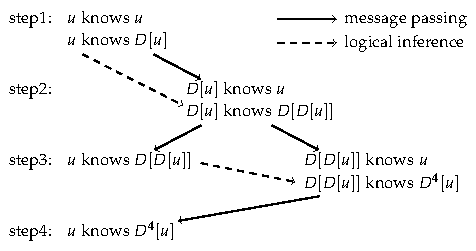
\includegraphics[width=0.75\textwidth]{figures/d4u.pdf}
 \caption{Interpretation of the derivation of $\forall u.\,\knows{u}{D^4[u]}$}
 \label{fig:d4u-msg}
\vspace{-2ex}\end{figure}

The derivation of $\forall u.\,\knows{u}{D^4[u]}$ is not unique, and there are derivations that correspond to inefficient solutions --- for example, there is also a derivation for the six-round solution based on request-reply conversations.
However, when searching for derivations, our algorithm will minimize the number of rounds of communication, as explained below.

\textbf{The compiling algorithm}:
The algorithm starts from a proposition $\forall u.\,\knows{v(u)}{e(u)}$.
%Later we will show that only considering these two patterns is enough.
The key problem here is to choose a proper $w(u)$ so that, by applying the message passing axiom backwards, we can get two potentially simpler new target propositions $\forall u.\,\knows{w(u)}{e(u)}$ and $\forall u.\,\knows{w(u)}{v(u)}$ and solve them respectively.
The range of such choices is in general unbounded, but our algorithm considers only those simpler than $v(u)$ or $e(u)$.
More formally, we say that $a$~is a \emph{subpattern} of~$b$, written $a \preceq b$, exactly when $b$~is a consecutive field access expression starting from~$a$.
%i.e., $b = \vec C[a]$ for a (possibly empty) chain $\vec C$ of fields.
For example, $u$~and $D[u]$ are subpatterns of $D[D[u]]$, while they are all subpatterns of $D^3[u]$.
The range of intermediate vertices we consider is then $\mathrm{Sub}(e(u), v(u))$, where $\mathrm{Sub}$ is defined by
\[ \mathrm{Sub}(a, b) = \{\,c \mid c \preceq a \mathrel\text{or} c \prec b \,\} \]
We can further simplify the new target propositions with the following function before solving them:
\[
\mathit{generalize}(\forall u.\,\knows{a(u)}{b(u)}) =
\begin{cases}
\forall u.\,\knows{u}{(b(u)/a(u))} & \text{if~} a(u) \preceq b(u) \\
\forall u.\,\knows{a(u)}{b(u)} & \text{otherwise}
\end{cases}
\]
where $b(u)/a(u)$ denotes the result of replacing the innermost $a(u)$ in $b(u)$ with~$u$.
(For example, $A[B[C[u]]]/C[u] = A[B[u]]$.)
This is justified because the original proposition can be instantiated from the new proposition.
(For example, $\forall u.\,\knows{C[u]}{A[B[C[u]]]}$ can be instantiated from $\forall u.\,\knows{u}{A[B[u]]}$.)

It is now possible to find an optimal solution with respect to the following inductively defined function $\mathit{step}$, which calculates the number of rounds of communication for a proposition:
\[ \setlength{\arraycolsep}{.2em}
\begin{array}{lcl}
\mathit{step}(\forall u.\,\knows{u}{u}) &=& 0 \\
\mathit{step}(\forall u.\,\knows{u}{\mathit{D}[u]}) &=& 0 \\
\mathit{step}(\forall u.\,\knows{v(u)}{e(u)}) &=& \displaystyle 1+ \min_{w(u)\in \mathrm{Sub}(e(u),v(u))}~\max(x, y) \\
\multicolumn{3}{l}{\quad\text{where}~x = \mathit{step}(\mathit{generalize}(\forall u.\,\knows{w(u)}{e(u)}))} \\
\multicolumn{3}{l}{\quad\phantom{\text{where}}~y = \mathit{step}(\mathit{generalize}(\forall u.\,\knows{w(u)}{v(u)}))}
\end{array} \]
It is straightforward to see that this is an optimization problem with optimal and overlapping substructure, which we can solve efficiently with memoization techniques.

With this powerful compiling algorithm, we are now able to handle any chain access expressions.
Furthermore, this algorithm optimizes the generated Pregel program in two aspects.
First, this algorithm derives a message passing scheme with a minimum number of supersteps, thus reduces unnecessary cost for launching supersteps in Pregel framework.
Second, by extending the memoization technique, we can ensure that a chain access expression will be evaluated exactly once even if it appears multiple times in a Palgol step, avoiding redundant message passing for the same value.


\subsection{Neighborhood Access}
\label{sec:neighboring-access}

Neighborhood access is another important communication pattern widely used in Pregel algorithms.
Precisely speaking, neighborhood access refers to those chain access expressions inside a non-nested loop traversing an edge list (\textbf{Nbr}, \textbf{In} or \textbf{Out}), where the chain access expressions start from the neighboring vertex.
The following code is a typical example of neighborhood access, which is a list comprehension used in the S-V algorithm program (Figure~\ref{fig:svppa-code}):
\begin{lstlisting}[basicstyle=\small\ttfamily,firstnumber=7]
    let t = minimum [ D[e.ref] | e <- Nbr[v] ]
\end{lstlisting}
Syntactically, a field access expression $D[e.\mathbf{ref}]$ can be easily identified as a neighborhood access.

The compilation of such data access pattern is based on the symmetry that if \emph{all} vertices need to fetch the same field of their neighbors, that will be equivalent to making all vertices send the field to all their neighbors.
This is a well-known technique that is also adopted by Green-Marl and Fregel, so we do not go into the details and simply summarize the compilation procedure as follows:
\begin{enumerate}
 \item In the first superstep, we prepare the data from neighbors' perspective.
  Field access expressions like $D[e.\mathbf{ref}]$ now become neighboring vertices' local fields $D[u]$.
  Every vertex then sends messages containing those values to all its neighboring vertices.
 \item In the next step, every vertex scans the message list to obtain all the values of neighborhood access, and then executes the loop according to the Palgol program.
\end{enumerate}

\section{Compiling Palgol Steps}
\label{sec:trans-step}

\begin{figure}
 \centering
 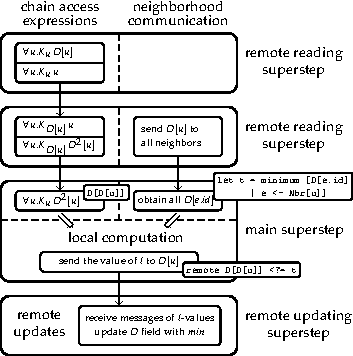
\includegraphics[width=0.75\textwidth]{figures/compile.pdf}
 \caption{Compiling a Palgol step to Pregel supersteps.}
 \label{fig:compiling-Palgol-step}
\vspace{-2ex}\end{figure}

Having introduced the compiling algorithm for remote data reads in Palgol, here we give a general picture of the compilation for a single Palgol step, as shown in \autoref{fig:compiling-Palgol-step}.
The computational content of every Palgol step is compiled into a \emph{main superstep}.
Depending on whether there are remote reads and writes, there may be a number of \emph{remote reading supersteps} before the main superstep, and a \emph{remote updating superstep} after the main superstep.

We will use the main computation step of the S-V algorithm program (lines 5--13 in \autoref{fig:svppa-code}) as a running example for explaining the compilation algorithm, which consists of the following four steps:

\begin{enumerate}
\item We first handle neighborhood accesss (for S-V algorithm, $D[e.\mathbf{ref}]$ at line~7).
As mentioned at the end of \autoref{sec:neighboring-access}, the evaluation of such expressions requires a sending superstep that provides all the remote data for the loops from the neighbors' perspective (for S-V algorithm, sending their $D$~field to all their neighbors).
This sending superstep is inserted as a remote reading superstep immediately before the main superstep.

\item We analyze the chain access expressions appearing in the Palgol step with the algorithm in \autoref{sec:consecutive}, and corresponding remote reading supersteps are inserted in the front.
(For S-V algorithm, the only interesting chain access expression is $D[D[u]]$, which induces two remote reading supersteps realizing a request-reply conversation.)
In addition, our handling of neighborhood access may introduce more chain accesses in the sending superstep, and message passing schemes should also be generated for those accesses.
(For S-V algorithm, the chain access introduced by neighborhood access is $D[u]$, which happens to be trivial.)

\item Having handled all remote reads, the main superstep receives all the values needed and proceeds with the local computation.
Since the local computational content of a Palgol step is similar to an ordinary programming language, the transformation is straightforward except for the handling of local writes.
In general, we need to create a separate copy of all the involved fields at the beginning of the superstep.
Then, during the superstep, all field reads are performed on the original fields, and all updates are on the copies.
Finally, we use the (possibly updated) values of the copies to update the original fields at the end of the superstep.

\item What remains to be handled is the remote updating statements, which require sending the updating values as messages to the target vertices in the main superstep.
(For S-V algorithm, there is one remote updating statement at line 10, requiring that the value of~$t$ be sent to $D[u]$.)
Then an additional remote updating superstep is added after the main superstep; this additional superstep reads these messages and updates each field using the corresponding remote updating operator.
(For S-V algorithm, the minimum of all the $t$-values received is assigned to field~$D$.)

\end{enumerate}

\section{Compiling Sequences and Iterations}
\label{sec:trans-iter}

We finally tackle the problem of compiling sequence and iteration, to assemble Palgol steps into larger programs.

A Pregel program generated from Palgol code is essentially a \emph{state transition machine} (STM) combined with computation code for each state.
In the simplest case, every Palgol step is translated into a ``linear'' STM consisting of a chain of states corresponding to the supersteps like those shown in \autoref{fig:compiling-Palgol-step}.
In general, a generated STM may be depicted as:
\begin{figure}[h]
 \centering
 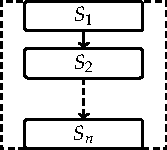
\includegraphics[width=0.25\textwidth]{figures/stm-general.pdf}
\end{figure}\\
where there are a start state and an end state, between which there can be more states and transitions, not necessarily having the linear structure.

\subsection{Compiling Sequences with STM Merging}

A sequence of two Palgol programs uses the first program to transform an initial graph to an intermediate one, which is then transformed to a final graph using the second program.
To compile the sequence, we first compile the two component programs into STMs; a composite STM is then built from these two STMs, implementing the sequence semantics.

\begin{figure}[t]
 \centering
 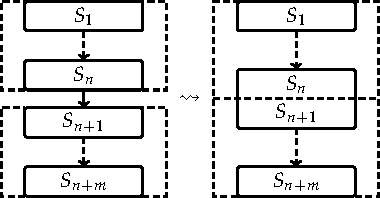
\includegraphics[width=0.6\textwidth]{figures/stm-seq.pdf}
 \caption{The compilation of sequence. A most straightforward way is shown on the left, and our compiler merges the states $S_n$ and $S_{n+1}$ and creates the STM on the right.}
 \label{fig:sequence}
\vspace{-2ex}\end{figure}

We illustrate the compilation in \autoref{fig:sequence}.
The left side is a straightforward way of compiling, and the right side is an optimized one produced by our compiler, with states $S_n$ and $S_{n+1}$ merged together.
This is because the separation of $S_n$ and $S_{n+1}$ is unnecessary:
every Palgol program describes an independent vertex-centric computation that does not rely on any incoming messages (according to our high-level model); correspondingly, our compilation ensures that the first superstep in the compiled program ignores the incoming messages.
We call this the \emph{message-independence} property.
Since $S_{n+1}$ is the beginning of the second Palgol program, it ignores the incoming messages, and therefore the barrier synchronization between $S_n$ and $S_{n+1}$ can be omitted.

\subsection{Compiling Iterations with STM Fusion}

Fixed-point iteration repeatedly runs a program enclosed by `\textbf{do}' and `\textbf{until} \ldots' until the specified fields stabilize.
To compile an iteration, we first compile its body into an STM, then we extend this STM to implement the fixed-point semantics.
The output STM is presented in \autoref{fig:fusion}, where the left one is generated by our general approach, and the right one performs the \emph{fusion optimization} when some condition is satisfied.

\begin{figure}[h]
 \centering
 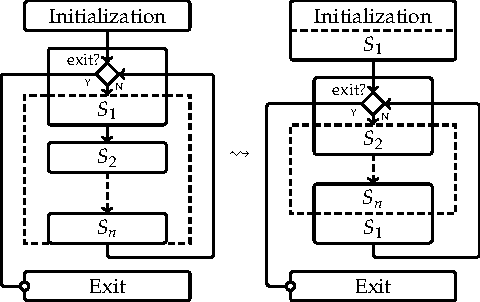
\includegraphics[width=0.75\textwidth]{figures/stm-opt.pdf}
 \caption{An STM for general iteration is shown on the left. The fusion optimization applies when the iteration body begins with a remote reading superstep ($S_1$), and yields the STM on the right.}
 \label{fig:fusion}
\vspace{-2ex}\end{figure}

Let us start from the general approach on the left.
Temporarily ignoring the initialization state, the STM implements a while loop:
first, a check of the termination condition takes place right before the state $S_1$: if the termination condition holds, we immediately enters the state \textit{Exit}; otherwise we execute the body, after which we go back to the check.
The termination check is implemented by an OR aggregator to make sure that every vertex makes the same decision:
basically, every vertex determines whether its local fields are changed during a single iteration by storing the original values before~$S_1$, and sends the result (as a boolean) to the aggregator, which can then decide globally whether there exists any vertex that has not stabilized.
What remains is the initialization state, which guarantees that the termination check will succeed in the first run, turning the while loop into a do-until loop.

There is a chance to reduce the number of supersteps in the loop body of the iteration STM when the first state $S_1$ of the loop body is a remote reading superstep (see \autoref{sec:trans-step}).
In this case, as shown on the right side of \autoref{fig:fusion}, the termination check is moved to the beginning of the second state $S_2$, and then the state $S_1$ is duplicated and attached to the end of both the initialization state and $S_n$.
This transformation ensures that, no matter from where we reach the state $S_2$, we always execute the code in $S_1$ in the previous superstep to send the necessary messages.
With this property guaranteed, we can simply iterate $S_2$ to $S_n$ to implement the iteration, so that the number of supersteps inside the iteration is reduced.
The only difference with the left STM is that we execute an extra $S_1$ attached at the end of $S_n$ when we exit the iteration.
However, it still correctly implements the semantics of iteration:
the only action performed by a remote reading superstep is sending some messages;
although unnecessary messages are emitted, the Palgol program following the extra $S_1$ will ignore all incoming messages in its first state, as dictated by the message-independence property.

\section{Combiner Optimization}
\label{sec:combiner}

Combiners are a mechanism in Pregel that may reduce the number of messages transmitted during the computation.
Essentially, in a single superstep, if all the messages sent to a vertex are only meant to be consumed by a reduce-operator (e.g., sum or maximum) to produce a value on that vertex, and the values of the individual messages are not important, then the system can combine the messages intended for the vertex into a single one by that operator, reducing the number of messages that must be transmitted and buffered.

In Pregel, combiners are not enabled by default, since ``there is no mechanical way to find a useful combining function that is consistent with the semantics of the user's \emph{compute()} method''~\cite{pregel}. %, and it is programmers' responsibility to provide an implementation for combiner.
On the other hand, Palgol's list comprehension syntax combines remote access and a reduce operator, and naturally represents such type of computation, which can potentially be optimized by a combiner.
A typical example is the SSSP program (line 7--8 in \autoref{fig:sssp-palgol}), where the distances received from the neighbors ($D[e.\mathbf{ref}]+e.\mathbf{val}$) are transmitted and reduced by the \textbf{minimum} operator.
Since the algorithm only cares about the minimum of the messages, and the compiler knows that nothing else is carried by the messages in that superstep, the compiler can automatically implement a combiner with the minimum operator to optimize the program.

\chapter{Customizing Pregel with Message Channel Interface}
\label{sec:custom}

In this chapter, we present our custom Pregel framework with the message channel interface, which brings more opportunities of reducing messages in computation.
The custom Pregel framework is designed to be a more efficient back-end for Palgol to fully take the advantages of Palgol's high-level semantics in program optimization, but it can also serve as an extended programming model for programmers to implement graph algorithms.
By introducing the message channels, our custom Pregel framework is more efficient to handle complex communication patterns in a graph algorithm.

\section{The Message Channel Interface}

In complex graph algorithms (like the S-V algorithm), a vertex may communication with different vertices in the same superstep, so that the messages for different purposes are mixed in the message list.
Although programmers can tag the messages to distinguish them, it is not an efficient solution.
Let us consider the scenario shown in \autoref{fig:multi-msg-example}.

\begin{figure}[th]
\centering
\begin{subfigure}[b]{0.45\textwidth}
 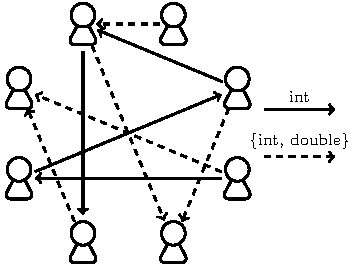
\includegraphics[width=\textwidth]{figures/multi-msg.pdf}
 \caption{space is wasted when tagging and encoding messages into the same type}
 \label{fig:multi-msg}
\end{subfigure}
\hspace{5pt}
\begin{subfigure}[b]{0.45\textwidth}
 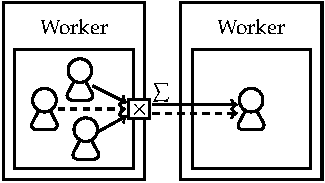
\includegraphics[width=\textwidth]{figures/comb-err.pdf}
 \caption{combiner optimization is not always applicable when different messages exist}
 \label{fig:comb-err}
\end{subfigure}
\caption{Two major problems when different messages exist in the same superstep}
\label{fig:multi-msg-example}
\end{figure}

Suppose there are two types of messages used in the same superstep, as shown in \autoref{fig:multi-msg}.
One is int type indicated by the solid arrow, and the other is a pair of int and double indicated by the dashed arrow.
In the original Pregel system, the single message type should be carefully chosen to be able to carry all types of messages used in the program.
Then, in this case, it must be at least a pair of int and double to envelope the largest possible message, which however causes a double word wasted for the messages using only int.
Moreover, the combiner optimization is not always applicable when different messages exist.
As mentioned in \autoref{sec:combiner}, the combiner is applicable when the messages are only meant to be consumed by a reduce-operator,
but when having different messages in a superstep, it is usually the case that only the messages for the same purpose can be combined.
In other words, the Pregel's combiner interface always combines \emph{all} the messages sent to the same destination vertex, but what we want is to combine a portion of the messages having the same tag, while leaving the other messages unchanged or optimized by other combiners.

The idea to solve these problem is to separate the communications into dedicated channels, instead of encoding messages on a unified message passing channel in current Pregel, so that the message type or the combiner for each communication channel can be specified individually.
Furthermore, with the separation of message channels, more communication patterns in graph algorithms can be easily integrated into our system, and specialized optimization can further improve the efficiency.
%Furthermore, by separating the messages for different purposes and studying the communication patterns individually, more efficient implementation of communication patterns can be easily integrated into our system.
To illustrate this, we show that the aggregator and the request-respond paradigm~\cite{pregelplus} can be regarded as special classes of message channels, and the S-V algorithm can thus be implemented more concisely in our framework.

The remaining problem is the system design to expose a reasonably simple interface for programmers to specify and use the message channels, which will be discussed in the next section.

\section{System Design \& Implementation}

In this part, we describe the details of our system design and the implementation of different types of the message channels, including the direct message channel with combiner, the aggregator, and the request-respond paradigm.

\subsection{The Communication Layer}

First of all, we use the term ``worker'' to represent a basic computing unit, which in general can be a machine or a thread/process in a machine, but in our system it just refers to a process.
When launching a graph processing task, multiple instances of workers are created, and each of them holds a disjoint portion of the graph (a subset of vertices along with their attributes and edge lists).
They corporate with each other to finish the graph computation in a distributed manner.

Workers share no memory with each other, but can exchange messages with other workers in batch through the underlying communication layer, which is implemented using the Message Passing Interface (MPI).
In particular, a worker maintains $M$ outgoing buffers (where $M$ is the number of workers allocated by the user), one for each worker in the cluster.
When a worker needs to send some data to another worker, it simply appends the data in the corresponding outgoing buffer, and it is until the end of a superstep that all the contents (not only this piece of data) in the outgoing buffers are finally delivered to their designated workers.
We accomplish it by the buffer exchange, which is implemented by $M$ rounds of pairwise communication among workers, while in each round every worker carefully selects a partner and exchanges the contents in the corresponding buffer through MPI's message passing primitives.
After the buffer exchange, the contents are further processed by the designated workers.

In the original Pregel system, the outgoing buffers can be seen as a single message channel which only stores the data that has the user-specified message type.
To support multiple message channels with different message types, our outgoing buffers are just raw char buffers which store serialized data, so that data with different types can be treated equally on our communication layer.
Besides, the messages are buffered by the message channels first, and in the end of each superstep, they are serialized to the outgoing buffers in batch to avoid the overhead of tagging the individual messages with type information for (de)serialization.
After the buffer exchange, the contents in the buffer have to be deserialized by the message channels in exactly the same order as they are serialized, so that the data can be correctly restored.

%Next, we discuss the implementation of three types of message channels: direct message passing channel, aggregator channel, and request-respond channel.

\subsection{Direct Message Passing \& Combiner}

Direct message passing is a standard mechanism provided by all Pregel frameworks.
In general, message passing can happen between any pair of vertices, but in some Pregel frameworks (like GraphX~\cite{graphx} and PowerGraph~\cite{powergraph}) vertices can only send direct messages to their neighbors in the input graph.
Allowing message passing between any pair of vertices is critical to make several graph algorithms~\cite{connectivity, pregelplus} converge fast,
so in our framework, we support the most general message passing, and the interfaces of direct message passing are shown in \autoref{fig:api-msg}.

\begin{figure}[ht]
\centering
\vspace{-2ex}
\begin{lstlisting}[basicstyle=\small\ttfamily,
numbers=none,language=c++,xleftmargin=0.1\textwidth]
template<typename VertexT, typename MsgT>
class V2V : public Serializable {
public:
   typedef typename VertexT::KeyT KeyT;
   typedef typename VertexT::HashT HashT;
   typedef void (*CombinerT)(MsgT &, const MsgT &);

   V2V(Worker<VertexT> *worker, const char *name,
       CombinerT comb = nullptr);

   void add_message(KeyT dst, const MsgT &msg);
   void send();
   bool empty();
   void reset();
   vector<vector<MsgT> >& collect();
};
\end{lstlisting}
\vspace{-2ex}
\caption{APIs for message passing channel}
\label{fig:api-msg}
\end{figure}

The class \texttt{V2V} represents the vertex-to-vertex communication, and it takes two type arguments: the vertex class (which includes the type of vertex identifier and a hash function), and the message type.
The constructor of class \texttt{V2V} further takes a worker, a string (for printing runtime information) and an optional combiner as arguments.
Programmers can add messages to the buffer, deliver the message after a superstep, check whether the message buffer is empty, reset the channel, and collect the messages sent in the previous superstep.

The implementation of the direct message passing is straightforward.
Messages are tagged with the destination vertex identifier and stored in the worker's local buffer.
They are serialized to the communication layer and sent to the destination when the \emph{send()} function is explicitly invoked.
If the combiner is specified, the combiner optimization is performed before serialization, by sorting and grouping the messages by the destination, and combining the messages for the same destination vertex by a user-specified binary function; otherwise the messages are sent directly.
After the buffer exchange, the message channels deserialize the messages and dispatch them to the receiving vertices on the current worker.

\subsection{Aggregator}

Aggregator is also a standard mechanism for all Pregel-like frameworks, which implements the global communication with a specified commutative and associative operator: it collects value from every active vertex, and then combines them to a final value by an operator.
Such communication pattern is particularly important for making a consensus or maintaining a consistent global state among all vertices during the computation.
The aggregator APIs are present in \autoref{fig:api-aggregator}.

\begin{figure}[ht]
\centering
\vspace{-2ex}
\begin{lstlisting}[basicstyle=\small\ttfamily,numbers=none,language=c++]
template<typename FinalT, typename LocalT, typename InputT>
class Aggregator : public Serializable {
public:
   typedef void (*LCombinerT)(LocalT &, const InputT &);
   typedef void (*FCombinerT)(FinalT &, const LocalT &);

   Aggregator(Sync *sync, LCombinerT lc, FCombinerT fc);

   void add_value(const InputT &v);
   void aggregate();
   const FinalT &result() const;

protected:
   LocalT& local();  // access the local value
   FinalT& final();  // access the final result

private:
   virtual void init_local() = 0;
   virtual void init_final() = 0;
};
\end{lstlisting}
\vspace{-2ex}
\caption{APIs for aggregator channel}
\label{fig:api-aggregator}
\end{figure}

The class \texttt{Aggregator} takes three type arguments: the type of input value, the type of the partial value stored on each worker, and the type of the final result.
Two combiners need to be specified by the programmer: one local combiner is to update the local value with an input value, and a global combiner is to update the final value by the partial values from other workers.
Meanwhile, programmers should also tell the aggregator how to initialize the local partial value and the final result before the aggregation.
Programmers can feed values, perform aggregation after a superstep, or read the final result of the aggregator.
The last thing to mention is that, unlike some Pregel frameworks where the aggregator automatically collects the value from all active vertices, in our system, programmers need to explicitly feed the values to the aggregator, making aggregator an independent mechanism to the vertex inactivation.
According to our experience, this makes some complex algorithms easy to implement.

The implementation of the aggregator is also straightforward.
On each worker, a local partial value is generated from the initial partial value and those input values passed to the aggregator, by using the local combiner.
Then, each worker sends its partial value to all other workers using the outgoing buffer interface, so that after the buffer exchange, every worker will receive the partial values from all other workers.
Finally, every worker uses the global combiner to reduce them to a final value.
In our implementation, the order of reducing the partial values is guaranteed to be the same on all workers, so that programmers can get a consistent final result with any global combiner.

\subsection{Request-Respond Paradigm}

Request-Respond Paradigm~\cite{pregelplus} is a two-phase communication pattern which can reduce the number of messages in the scenario where every vertex needs to fetch a remote vertex's attribute.
Since Pregel is based on ``message pushing'' that the sender should specify the receiver in message passing, such communication pattern has to be decomposed into a request and a response phase:
in the request phase, each vertex sends a request to a remote vertex, then in the consequent response phase, vertices may receive the requests from other vertices, and they respond a value to them.
In this communication pattern, the number of vertices that receive requests is usually much less than the number of active vertices in the graph, which gives a chance for message reduction.
The idea is to let the worker merge the requests for the same destination in the sending phase, so that any vertex will receive at most one request from each worker.
Then, a vertex just responds to each requesting worker with a value, instead of responding to individual vertices.
Finally, when the workers receive the responses (tagged with the responser's id), they dispatch the values to the requesting vertices.

Due to the extra information kept on the sending worker (for dispatching the responses), this optimization cannot be implemented by the direct message passing with combiner, thus it is regarded as a special communication pattern and implemented as a set of extended interfaces in Pregel\plus~\cite{pregelplus}.
The integration is however not convenient for programmer to use:
similar to the message passing and aggregator interface, Pregel\plus's request-respond interface is shared by the whole program and the type of response value is provided by the programmer at the beginning, therefore when multiple request-respond communications are required in the program, programmers should carefully arrange them in different supersteps (since in each superstep, a vertex can respond only one value), and encode them to a same type.
In contrast, in our custom Pregel framework, we just implement it as a special type of message channels, so programmers can specify each request-respond channel individually, making the implementation logic of graph algorithms extremely easy.
%Another remarkable difference is that, Pregel\plus uses an additional communication channel for request-respond paradigm, while our system implement the request-respond channel on top of the raw char buffer, which potentially reduce the number of message exchanges among workers.
The APIs for request-respond channel are presented in \autoref{fig:api-reqresp}.

\begin{figure}[ht]
\centering
\vspace{-2ex}
\begin{lstlisting}[basicstyle=\small\ttfamily,numbers=none,language=c++]
template<typename VertexT, typename ValT>
class ReqResp : public Serializable {
public:
   typedef typename VertexT::KeyT KeyT;
   typedef typename VertexT::HashT HashT;

   ReqRes(Worker<VertexT> *worker, const char *name);

   void add_request(int index, KeyT dst);
   void request();
   void respond(const vector<ValT> &val);
   void collect(vector<ValT> &val);
   void reset();
};
\end{lstlisting}
\vspace{-2ex}
\caption{APIs for request-respond channel}
\label{fig:api-reqresp}
\end{figure}

The class \texttt{ReqResp} takes two type arguments: the vertex class (which includes the type of vertex identifier and a hash function), and the message type.
In the request phase, programmers can add requests to the buffer by invoking the function \emph{add\_request(index, dst)}, where \emph{index} is the unique index of the requesting vertex on current worker, and \emph{dst} is the destination vertex identifier.
Here, using the index of the requester (which is exposed to programmers) can improve the performance, since we can feed the responses to the requesters directly through the index, which avoids the expensive table lookup in the response phase.
Next, \emph{request()} should be invoked after all requests are added, to let the system preprocess the requests and deliver them after the current superstep.
The respond function \emph{respond(val)} is then invoked in the next superstep on all workers, where \emph{val} stores the values to respond for each vertex.
Note that this mechanism is implemented in a passive way: although every vertex need to prepare a value for responding the requests, the system will only access the values from the vertices that receive requests.
Finally, after the responses are delivered, we collect the results using the \emph{collect(val)} function, which returns an array containing the requested value for each vertex.

Here we explain the implementation of the request-respond message channel in detail.
First, on each worker, we buffer all the requests, which can be seen as a list of $\langle dst,index\rangle$ pairs where $index$ is the requesters' index on this worker.
In the \emph{request()} function, we sort all the requests and extract the distinct destinations from the requests, and furthermore, for each distinct destination vertex id, we keep the index of its first occurrence in the request list, so we obtain the $\langle dst_{unique},index_{req}\rangle$ pairs.
This list is further split into $M$ request lists depending on where the destination vertex locates (vertex $dst$ locates on worker $w$ where $w=hash(dst)$).
The exchange of the requests and responses are straightforward.
After the response values are received, we can get the tuples containing $\langle dst_{unique},index_{req},value\rangle$ by merging the responses with the request lists.
Finally, using $dst_{unique}$ and $index_{req}$, we can efficiently find all the requests in the sorted request buffer that have destination $dst_{unique}$, then using the index information, we efficiently feed the $value$ to all requesting vertices.

\begin{comment}
Our implementation slightly differs from the implementation of Pregel\plus in two aspects.
First, when programmers send requests in a certain superstep, Pregel\plus actually performs the request and response phase consecutively, so that the programmers can get the response in the next superstep.
The reason is that, Pregel\plus assumes that the requesters always want to fetch a remote vertex's attribute, so by providing a \emph{respond()} interface in class \texttt{Vertex}, vertices can respond that attributes to the requesters and Pregel\plus can automate the response phase.
Instead, in our system, the request phase and respond phase happen in individual supersteps, and the response value can be generated by any user-specified computation.
\end{comment}

\section{Programming Interface}

Programs written on our custom Pregel are quite different from those written in Pregel.
We summarize the differences as follows:
\begin{itemize}\setlength\itemsep{0em}
\item
 First, in Pregel systems, the computation are supposed to be implemented on each vertex, but our custom Pregel framework requires the computation to be implemented on the worker.
 However, it is just a choice of design and will not change the vertex-centric programming model.
 By exposing the vertices stored on each worker to the programmers, programmers are actually programming in a very similar way as in any other Pregel systems.
\item
 Second, Pregel introduces the ``voting to halt'' mechanism for terminating the computation (and in some cases for program optimization), but we provide a much simpler way for termination.
 In particular, the user-defined \emph{compute()} function returns a boolean value indicating the current worker's local decision of termination, and the whole computation terminates when all workers decide to stop.
\item
 Third, in our custom Pregel system, message passing, aggregator and request-respond paradigm are just three types of communication channels, so programmers can define various instances of communication channels, specify the message types (and combiners) individually, and explicitly manage them during the computation according to their APIs.
\item
 Forth, the indexes of the vertices are now exposed to the programmers, so they can use sort of global arrays defined on the worker to store the attributes of the vertices.
 Although this feature seems to give too much obligations to the users and may make the system hard to use, it is however a useful feature for code generation, and thus is kept in our current implementation.
 We will give a concrete example in \autoref{sec:sv-impl}.
\end{itemize}

To better illustrate how our system works, we use the following pseudo code to describe the computation on each worker in \autoref{fig:semantics-worker}:

\begin{figure}[ht]
\centering
\vspace{-2ex}
\begin{lstlisting}[basicstyle=\small\ttfamily,numbers=none,xleftmargin=0.1\textwidth]
do
   bool ret = this.compute(); // defined by user
   stop = all_stop(ret);      // reach a consensus
   if (!stop)
      exchange the messages;  // communication
until (stop);
\end{lstlisting}
\vspace{-2ex}
\caption{Pseudo code for describing the execution of each worker}
\label{fig:semantics-worker}
\end{figure}

\section{Example: The S-V Algorithm}

As a running example, let's see how the S-V algorithm~\cite{connectivity} is implemented in our custom Pregel system.
The Palgol's high-level description is shown in \autoref{fig:svppa-code}, and according to the compilation algorithm presented in \autoref{sec:compilation}, the compilation result is shown in figure \autoref{fig:full}, which contains four supersteps.

\begin{figure}[ht]
 \centering
 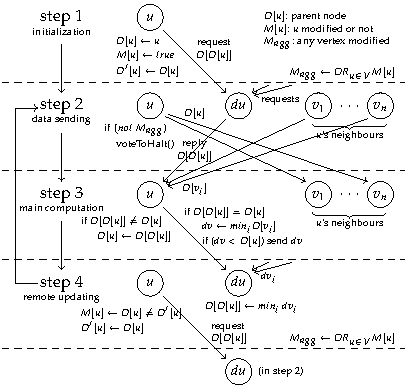
\includegraphics[width=0.8\textwidth]{figures/svppa.pdf}
 \caption{The compilation result of S-V algorithm}
 \label{fig:full}
\end{figure}

\subsection{Declaration of Message Channels}

Let us first consider what kind of message channels are needed for implementing the S-V algorithm.
From the compilation result of Palgol compiler, we can find three message channels, which are:
\begin{itemize}
\item
 The request-respond message channel to calculate $D[D[u]]$ in the main step.
 The request phase happens in both step 1 and step 4, while the response phase only appears in step 2.
 By following the state transition machine, we can easily verify that vertices always send the requests in the previous step of the response phase.
\item
 The direct message passing channel to collect all the neighbors' pointers to their parent, which happens between step 2 and step 3.
 The message type is the same as the type of vertex identifier.
 Note that, this message passing channel can be optimized by a combiner that calculates the minimum of the messages, since each vertex only cares about the minimum of neighbors' parent id.
\item
 The direct message passing channel to implement the remote writes in line 10 of the Palgol program shown in \autoref{fig:svppa-code}, which happens between step 3 and step 4.
 The message type is the same as the type of vertex identifier, and it can be optimized by a combiner as well, since the vertex receiving the remote writes only cares about the minimum value of the messages.
\end{itemize}

In the program, we use the variable \textit{grandparent} to represent the pointer jumping channel for calculating the grandparent (parent's parent) of every vertex, and use the variables \textit{neighbor} and \textit{remote} to represent the direct message channels for collecting all neighbors' pointer and remote writes.
The code shown in \autoref{fig:sv-declaration} defines the class \texttt{SVWorker} for implementing the S-V algorithm, declares the message channels in this class, and initializes them in the constructor.
There are three message channels defined here: two direct message channels with messages of integer message type, and one request-respond channel with integer response value.

\begin{figure}[ht]
\centering
\vspace{-2ex}
\begin{lstlisting}[basicstyle=\small\ttfamily,numbers=none,language=c++,
xleftmargin=0.1\textwidth]
typedef Vertex<int, vector<int> > VertexT;
class SVWorker : public Worker<VertexT> {
private:
   // declaration of message channels
   V2V<VertexT, int> neighbor, remote;
   ReqResp<VertexT, int> grandparent;
public:
   SVWorker():  // initialization
      grandparent(this, "Pointer Jumping"),
      neighbor(this, "Neighborhood", c_min),
      remote(this, "Remote Write", c_min) {}
   // the user-specified compute function
   bool compute() { .. }
};
\end{lstlisting}
\vspace{-2ex}
\caption{Declaration of message channels for S-V}
\label{fig:sv-declaration}
\end{figure}

%In the next section, we will show how to use these message channels in the \emph{compute()} function for data communication.

\subsection{Implementation of Individual Supersteps}
\label{sec:sv-impl}

Having declared the message channels, next is to consider how to implement each superstep in the worker's \emph{compute()} function.
%The \emph{compute()} function is a virtual member function of class \texttt{Worker} that should be implemented by the programmers.
It is a well-know technique that we can implement an algorithm with many computation stages (like the S-V algorithm) in a single \emph{compute} function, by referring to a global state and executing different code accordingly.
Here we use a local variable \texttt{step} to simulate the global state, but it is guaranteed to be consistent among all workers by our implementation.

\begin{figure}[ht]
\centering
\vspace{-2ex}
\begin{lstlisting}[basicstyle=\small\ttfamily,language=c++]
bool compute() {
   .. // code for other supersteps
   if (step == 3) {
      // collect messages from the previous superstep
      auto &msgs = neighbor.collect();
      // collect responses from parent vertices
      grandparent.collect(D2);
      // enter vertex-centric computation
      for (int u = 0; u < numv(); u++) {
         if (D2[u] == D[u]) {
            int t = (msgs[u].empty() ? INF : 
               *min_element(msgs[u].begin(), msgs[u].end()));
            if (t < D[u])  // send an update to parent
               remote.add_message(D[u], t);
         } else
            D[u] = D2[u];
      }
      remote.send(); // deliver messages after this step
      step = 4;      // state transition
      return false;  // don't terminate
   }
   .. // code for other supersteps
}
\end{lstlisting}
\vspace{-2ex}
\caption{The implementation of step 3 for the S-V algorithm}
\label{fig:sv-step3}
\end{figure}

\autoref{fig:sv-step3} shows the implementation of the main step (step 3) for the S-V algorithm.
Before entering the vertex-centric computation, programmers should explicitly collect the messages form the previous superstep.
So in lines 4--7, we collect the messages from the neighbors in $msgs$ (which stores each vertex's message list) and collect the ids of grandparents in $D2$ (a list storing each vertex's grandparent).
After all the necessary messages are collected, we enter the vertex-centric computation by writing the for loop in line 9--17, in which $numv()$ is the number of vertices on the worker.
Then, $D$ is an array storing the current parent's id for each vertex on this worker (which is calculated in previous supersteps), and we just use the raw index $u$ to access the attributes of the vertices.
Then, since $D2$ stores the grandparent's id and $D$ stores the parent's id, the expression \texttt{D2[u] == D[u]} in line 10 checks whether a vertex's parent is a root.
If it is the case, we calculate the minimum of neighbors' parent id as $t$, and modify $u$'s parent's pointer with $t$, which is achieved by adding a message $t$ to \texttt{D[u]} by the remote updating channel $remote$;
the messages buffered by the \emph{remote} channel are eventually delivered by the \emph{send()} function on line 19, so that the messages are expected to reach the destinations in step 4, according to the state transition in line 19.
If $u$'s parent is not a root vertex, then current vertex $u$ modifies its pointer $D$ to $u$'s grandparent $D2[u]$ by an assignment in line 16.
Finally, in line 20, we return \texttt{false} indicating that the computation should continue after current superstep ends.

The way to implement the other supersteps are basically the same, by collecting the messages first, performing the vertex-centric computation next, and then delivering the necessary messages for the next superstep, changing the global state, and returning a proper value indicating whether the computation stops.
In this example, we can see that our custom Pregel framework can intuitively implement complex Pregel algorithms with multiple communication channels.
Furthermore, we make the \emph{neighbor} channel and \emph{remote} channel to be optimized by the minimum combiner, which is natural in our system but impossible to achieve in other Pregel frameworks.

\section{Compiling Palgol to Message Channel Interface}

In this section, we will show that the message channel interface is a perfect match for Palgol, since high-level communication patterns can be recognized just syntactically in Palgol.
Basically, Palgol has four classes of remote access patterns: chain access, neighborhood access, remote writes and global communication in the termination condition of iterations.
Here we discuss how they map to the message channel interfaces, and sketch a transformation from Palgol to our custom Pregel system as well.

\textbf{Chain access}: In Palgol, chain access refers to a nested global field access expression, where programmers start from the current vertex and consecutively follow a reference to reach some remote vertex, and finally read that remote vertex's field.
Syntactically, chain has the form of \texttt{A[B[..Z[u]]]} where $u$ is the current vertex and the fields involved (except the outermost one) have the type of vertex id.
A naive implementation of chain access is to create a direct message passing channel without combiner for each message passing axiom (in \autoref{sec:consecutive}), but sometimes we can implement a chain access by the request-respond paradigm (like \texttt{D[D[u]]} in the S-V algorithm).
Essentially, chain access expressions in the form of \texttt{A[B[u]]} exactly describes a request-respond communication, where \texttt{B[u]} is the destination of the request emitted by every vertex, and $A$ field is the expected respond value.
In the Palgol compiler, we can specialize the implementation of chain access in such form by a request-respond channel.

\textbf{Neighborhood access}: List comprehension is the basic syntax in Palgol to describe remote access from all neighboring vertices, and we have already mentioned the combiner optimization in \autoref{sec:combiner}.
In Palgol compiler, we just create a direct message passing channel for list comprehension, and the combiner can be directly derived from Palgol's build-in function.
For loops in Palgol is implemented in a similar way, but the combiner optimization is disabled.

\textbf{Remote writes}: Remote writes in Palgol also compile to the direct message passing channel.
Moreover, according to the semantics of remote write described in \autoref{sec:palgol-model}, programmers must specify an ``accumulative'' assignment to avoid the potential non-determinism when updating a remote field (except the \texttt{.append(..)}).
In Palgol, any ``accumulative'' assignment can be optimized by a combiner on its message channel.
For example, the assignment operator \texttt{-=} subscribes all the received values from a remote field, and a ``sum'' combiner is obviously effective in this case.
We can just encode the rules in the Palgol compiler, so that remote writes in Palgol can always be efficiently implemented on our custom Pregel system.

\textbf{Termination conditions}: Termination conditions (indicated by the keywords ``forall'', ``exists'', ``fix'') in do-until iterations are naturally translated to aggregator channels with AND (or OR) operation, which collects values from all vertices and reduce to a final value using either AND or OR.

The translation form Palgol to our custom Pregel system is even simpler.
The skeleton of the algorithm is basically identical to the one described in \autoref{sec:compilation}, while the details are greatly simplified.
Message channels are now separately specified and managed, so we no longer need to consider the message encoding or decoding when implementing remote access, and the verbose checking of the applicability of combiner optimization is no need.
Attributes of the vertices can be defined as global arrays on the worker, which become more close to Palgol's global array syntax.
%Finally, we note that our custom Pregel framework is designed to be a better backend for Palgol, while providing such user interface is just some .
It is a future work to extends our compiler to compile Palgol programs to our custom Pregel framework.
%Since we haven't implement the compiler yet, we manually implement all the algorithms introduced in this thesis on our custom Pregel according to their high-level description in Palgol, which can be found in our repository\footnote{Our custom Pregel system with all implementation codes and examples is available at \url{https://bitbucket.org/zyz915/pregel}.}.

\chapter{Evaluation}
\label{sec:evaluation}

In this chapter, we are going to answer the following two questions: whether the programs written in Palgol is comparable to the ones written by human, and what's the essential difference between our compiled code and the human written ones with best effort.
We present the performance evaluation and an analysis on implementation quality in this part.

\section{Methodology}

%We evaluate and compare the performance of the Pregel programs generated by our Palgol compiler, the manually coded Pregel programs, and the manually transformed programs using our custom Pregel system over large real-world graphs.
%The experiments are conducted on an Amazon EC2 cluster with 16 nodes (instance type is m4.large), each containing 2 vCPUs and 8G memory.

%Our compilation algorithm for remote access combined with existing optimization techniques makes the efficiency of Palgol code comparable to hand-written code.
Currently, we compile Palgol code to Pregel\plus\footnote{\url{http://www.cse.cuhk.edu.hk/pregelplus}}, which is a lightweight open-source implementation of Pregel written in C\plusplus.
Note that Palgol does not target a specific Pregel-like system.
Instead, by properly implementing different backends of the compiler, Palgol can be transformed into any Pregel-like system, as long as the system supports the basic Pregel interfaces including message passing between arbitrary pairs of vertices and aggregators.
%, though any Pregel-like system can be used.
We have implemented the following six graph algorithms on Pregel\plus's basic mode, which are:
\begin{itemize}\setlength\itemsep{-0.4em}
 \item PageRank~\cite{pregel}
 \item Single-Source Shortest Path (SSSP)~\cite{pregel}
 %\item Randomized Bipartite Matching (BM)~\cite{pregel}
 \item Strongly Connected Components (SCC)~\cite{connectivity}
 \item Shiloach-Vishkin Connected Component Algorithm (S-V)~\cite{connectivity}
 \item List Ranking Algorithm (LR)~\cite{connectivity}
 \item Minimum Spanning Forest (MSF)~\cite{boruvka}
 %\item Randomized Graph Coloring (GC)~\cite{optimizing}
 %\item Approximate Maximum Weight Matching (MWM)~\cite{optimizing}
 %\item Triangle Counting (TC)~\cite{triangle}
\end{itemize}
Among these algorithms, SCC, S-V, LR and MSF are non-trivial ones which contain multiple computing stages.


In our performance evaluation, we use three real-world graph datasets (Facebook\footnote{https://archive.is/o/cdGrj/konect.uni-koblenz.de/networks/facebook-sg}, Wikipedia\footnote{http://konect.uni-koblenz.de/networks/dbpedia-link}, USA\footnote{http://www.dis.uniroma1.it/challenge9/download.shtml}) and one synthetic graph, where the detailed information is listed in Table~\ref{tab:datasets}.
The experiments are conducted on an Amazon EC2 cluster with 16 nodes (whose instance type is m4.large), each containing 2 vCPUs and 8G memory.
Each algorithm is run on the type of input graphs to which it is applicable (PageRank on directed graphs, for example) with 4 configurations, where the number of cores changes from 4 to 16.
We measure the execution time and the number of supersteps for each experiment, and all the results are averaged over three repeated experiments.

\begin{table}[t]
 \centering
 \caption{Datasets for Performance Evaluation}
 \label{tab:datasets}
 \resizebox{\textwidth}{!}{
 \begin{tabular}{c|c|c|c||l}
  \hline
  \textbf{Dataset} & \textbf{Type} & $|V|$ & $|E|$ & \multicolumn{1}{c}{Description} \\
  \hline\hline
  Wikipedia & Directed & 18,268,992 & 172,183,984 & the hyperlink network of Wikipedia \\
  \hline
  Facebook & Undirected & 59,216,214 & 185,044,032 & a friendship network of the Facebook \\
  \hline
  USA & Weighted & 23,947,347 & 58,333,344 & the USA road network \\
  \hline
  Random & Chain & 10,000,000 & 10,000,000 & a chain with randomly generated values \\
  \hline
 \end{tabular}}
\end{table}

\section{Performance Evaluation}

The runtime results of our experiments are summarized in \autoref{tab:exec}.
Remarkably, for most of these algorithms (PageRank, SCC, S-V and MSF), we observed highly close execution time on the compiler-generated programs and the manually implemented programs,
with the performance of the Palgol programs varying between a $2.53\%$ speedup to a $6.42\%$ slowdown.

For SSSP, we observed a slowdown up to $29.55\%$.
The main reason is that the human-written code utilizes Pregel's \textit{vote\_to\_halt()} API to deactivate converged vertices during computation;
this accelerates the execution since the Pregel system skips invoking the \emph{compute()} function for those inactive vertices, while in Palgol, we check the states of the vertices to decide whether to perform computation.
Similarly, we observed a $24\%$ slowdown for LR, since the human-written code deactivates all vertices after each superstep, and it turns out to work correctly.
While voting to halt may look important to efficiency, we would argue against supporting voting to halt as is, since it makes programs impossible to compose:
in general, an algorithm may contain multiple computation stages, and we need to control when to end a stage and enter the next; voting to halt, however, does not help with such stage transition, since it is designed to deactivate all vertices and end the whole computation right away.

\begin{table}[t]
 \centering
 \caption{Comparison of the Execution Time (in Seconds)}
 \label{tab:exec}
 \resizebox{\textwidth}{!}{
 \begin{tabular}{c|c||c|c||c|c||c|c||c|c||c}
  \hline
  \multirow{2}{*}{\textbf{Dataset}} & \multirow{2}{*}{\textbf{Algorithm}} & \multicolumn{2}{c||}{4 cores} & \multicolumn{2}{c||}{8 cores} & \multicolumn{2}{c||}{12 cores} & \multicolumn{2}{c||}{16 cores} & \multirow{2}{*}{Comparison} \\
  \cline{3-10}
  & & Pregel\plus & Palgol & Pregel\plus & Palgol & Pregel\plus & Palgol & Pregel\plus & Palgol & \\
  \hline\hline
  \multirow{3}{*}{Wikipedia} & SSSP & 8.33 & 10.80 & 4.47 & 5.61 & 3.18 & 3.83 & 2.41 & 2.85 & 18.06\% -- 29.55\% \\
  \cline{2-11}
  & PageRank & 153.40 & 152.36 & 83.94 & 82.58 & 61.82 & 61.24 & 48.36 & 47.66 & -1.62\% -- 2.26\% \\
  \cline{2-11}
  & SCC & 177.51 & 178.87 & 85.87 & 86.52 & 61.75 & 61.89 & 46.64 & 46.33 & -0.66\% -- 0.77\% \\
  \hline
  Facebook & S-V & 143.09 & 142.16 & 87.98 & 86.22 & 67.62 & 65.90 & 58.29 & 57.49 & -2.53\% -- -0.65\% \\
  \hline
  Random & LR & 56.18 & 64.69 & 29.58 & 33.17 & 19.76 & 23.48 & 14.64 & 18.16 & 12.14\% -- 24.00\% \\
  \hline
  USA & MSF & 78.80 & 82.57 & 43.21 & 45.98 & 29.47 & 31.07 & 22.84 & 24.29 & 4.79\% -- 6.42\% \\
  \hline
 \end{tabular}}
\end{table}

\section{Analysis on Implementation Quality}

The generated programs and the human written ones basically implement the same algorithms.
However, by directly comparing the execution time, we cannot say much about the implementation quality, since the execution time is actually affected by many reasons.
Here, we compare the number of supersteps used by our Palgol program and the hand-written code.
The number of supersteps measures the \emph{compactness} of the implementation, where a compact program is achieved by carefully analyzing the data dependencies and arranging the computation in a certain way so that the number of barrier synchronization is minimized.
Since barrier synchronization is known as an expensive operation, compactness is an important measurement of the implementation quality.
We present the results in \autoref{tab:steps}.

The generated programs for PageRank and S-V are almost identical to the hand-written versions,
while some subtle differences exist in the rest four algorithms.
For SCC, the whole algorithm is a global iteration with several iterative sub-steps, and the human written code can exit the outermost iteration earlier by adding an extra assertion in the code (like a \textbf{break} inside a \textbf{do ... until} loop).
Such optimization is not supported by Palgol currently, which results in a few additional supersteps performing the forward/backward propagation and some post-processing.
For MSF, the human written code optimizes the evaluation of a special expression $D[D[u]] \shorteqq u$ to only one round of communication, while Palgol's strategy always evaluates the chain access $D[D[u]]$ using a request followed by and a reply step, and then compares the result with $u$.
From \autoref{tab:exec}, we can see that these differences are however not critical to the performance, but the number of supersteps slightly increases.
For SSSP and LR, the human written code uses the voting to halt mechanism, therefore reduces one superstep compared to the generated code that uses aggregator.
As mentioned before, the slowdown of these two programs is mainly due to the vertex inactivation, while the impact of early termination is actually negligible.

\begin{table}[t]
 \centering
 \caption{Comparison of the Number of Supersteps}
 \label{tab:steps}
 \begin{tabular}{c|c|c|c|c}
  \hline
  \textbf{Dataset} & \textbf{Algorithm} & Pregel\protect\plus & Palgol & Comparison \\
  \hline\hline
  \multirow{3}{*}{Wikipedia} & SSSP & 49 & 50 & $2.04$\% \\
  \cline{2-5}
  & Pagerank & 32 & 32 & $0$\% \\
  \cline{2-5}
  & SCC & 1269 & 1278 & $0.71$\% \\
  \hline
  USA & MSF & 167 & 192 & $14.97$\% \\
  \hline
  Facebook & S-V & 14 & 14 & $0$\% \\
  \hline
  Random & LR & 51 & 52 & $1.96$\% \\
  \hline
 \end{tabular}
\end{table}

\begin{comment}
\centering
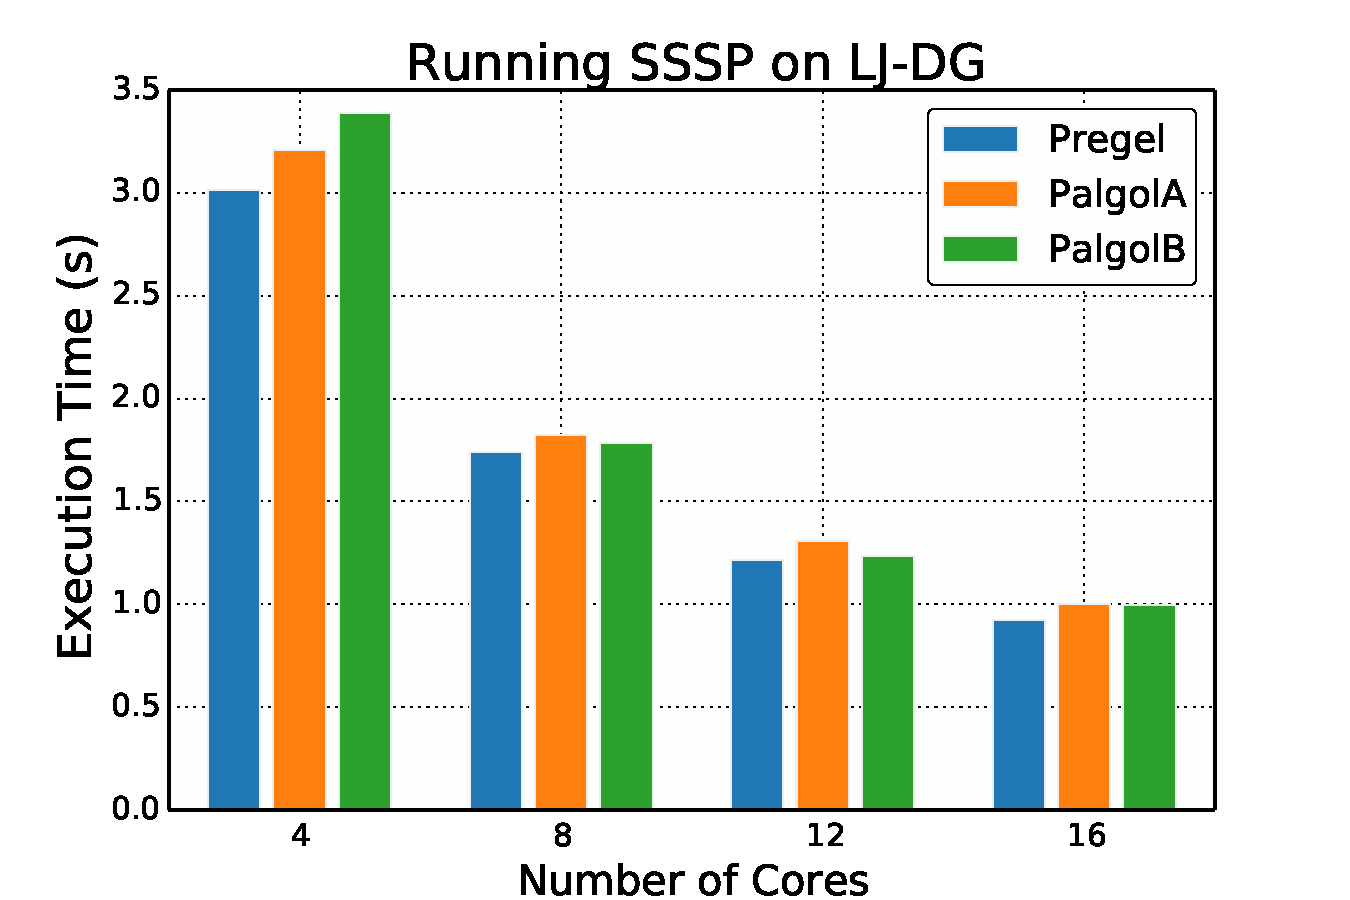
\includegraphics[width=0.48\textwidth]{plot/exec_sssp_LJ-DG.pdf}
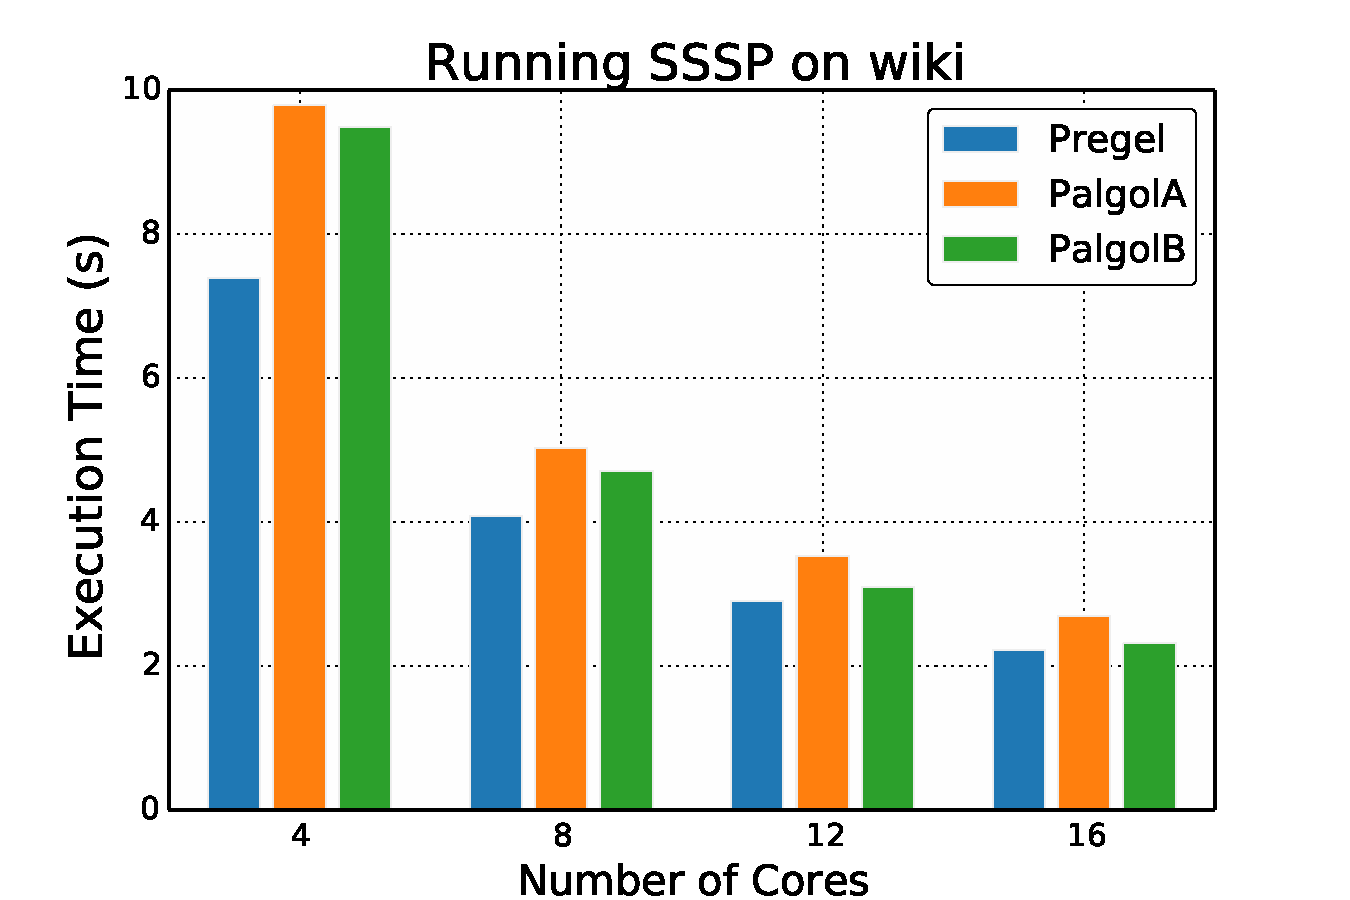
\includegraphics[width=0.48\textwidth]{plot/exec_sssp_wiki.pdf}
\\
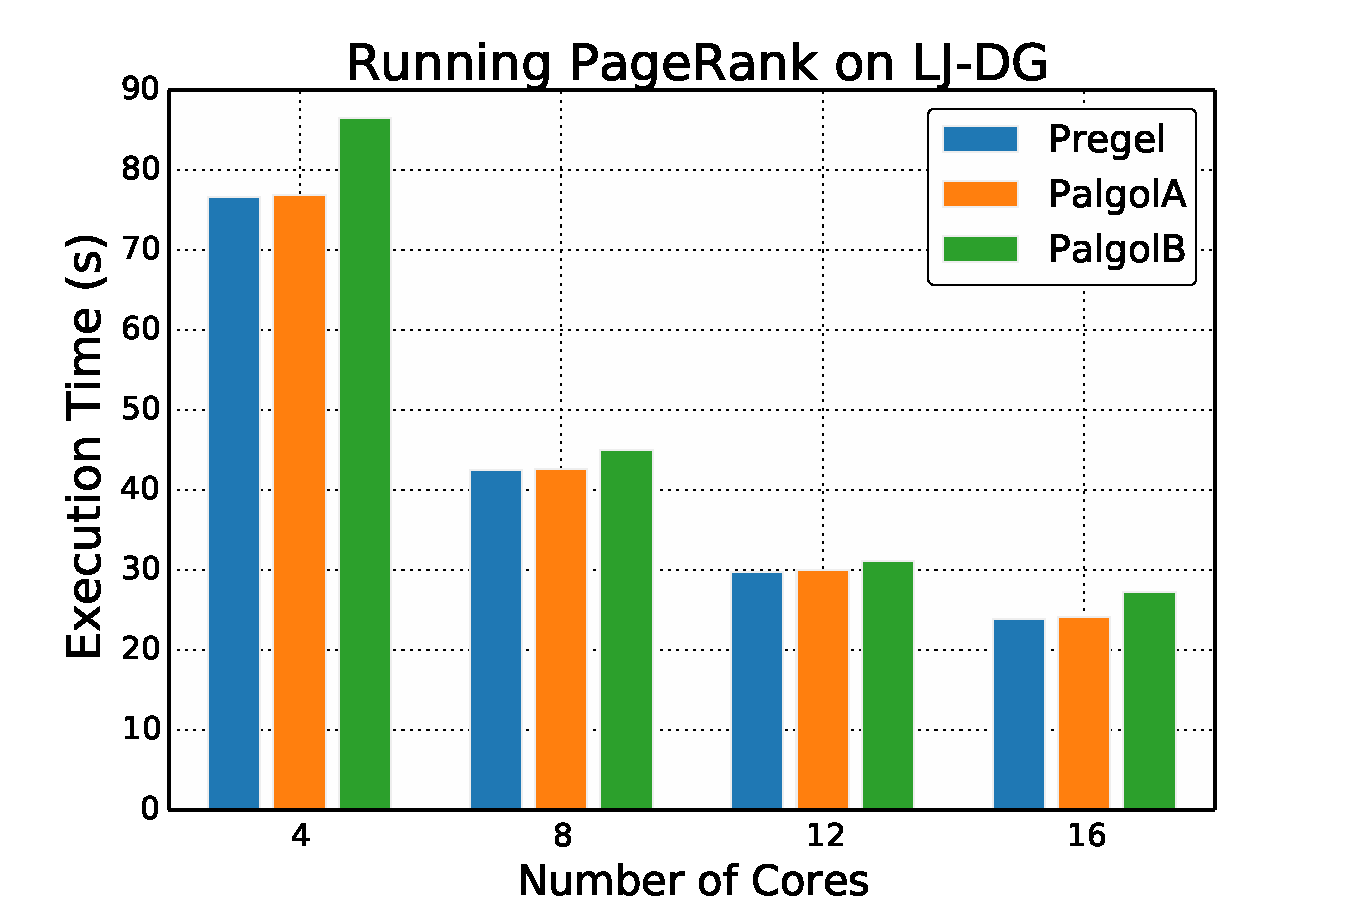
\includegraphics[width=0.48\textwidth]{plot/exec_pagerank_LJ-DG.pdf}
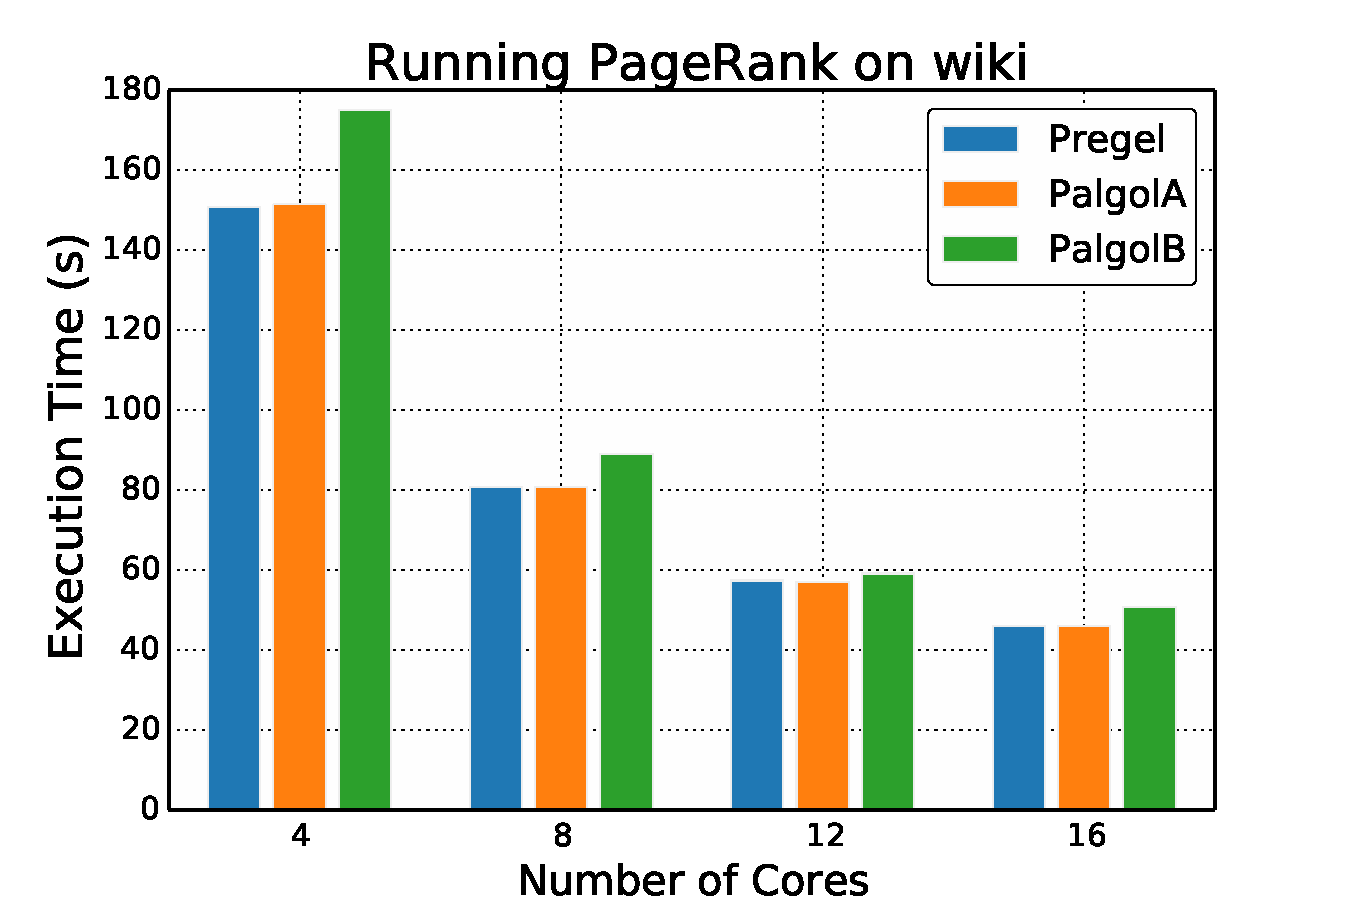
\includegraphics[width=0.48\textwidth]{plot/exec_pagerank_wiki.pdf}
\\
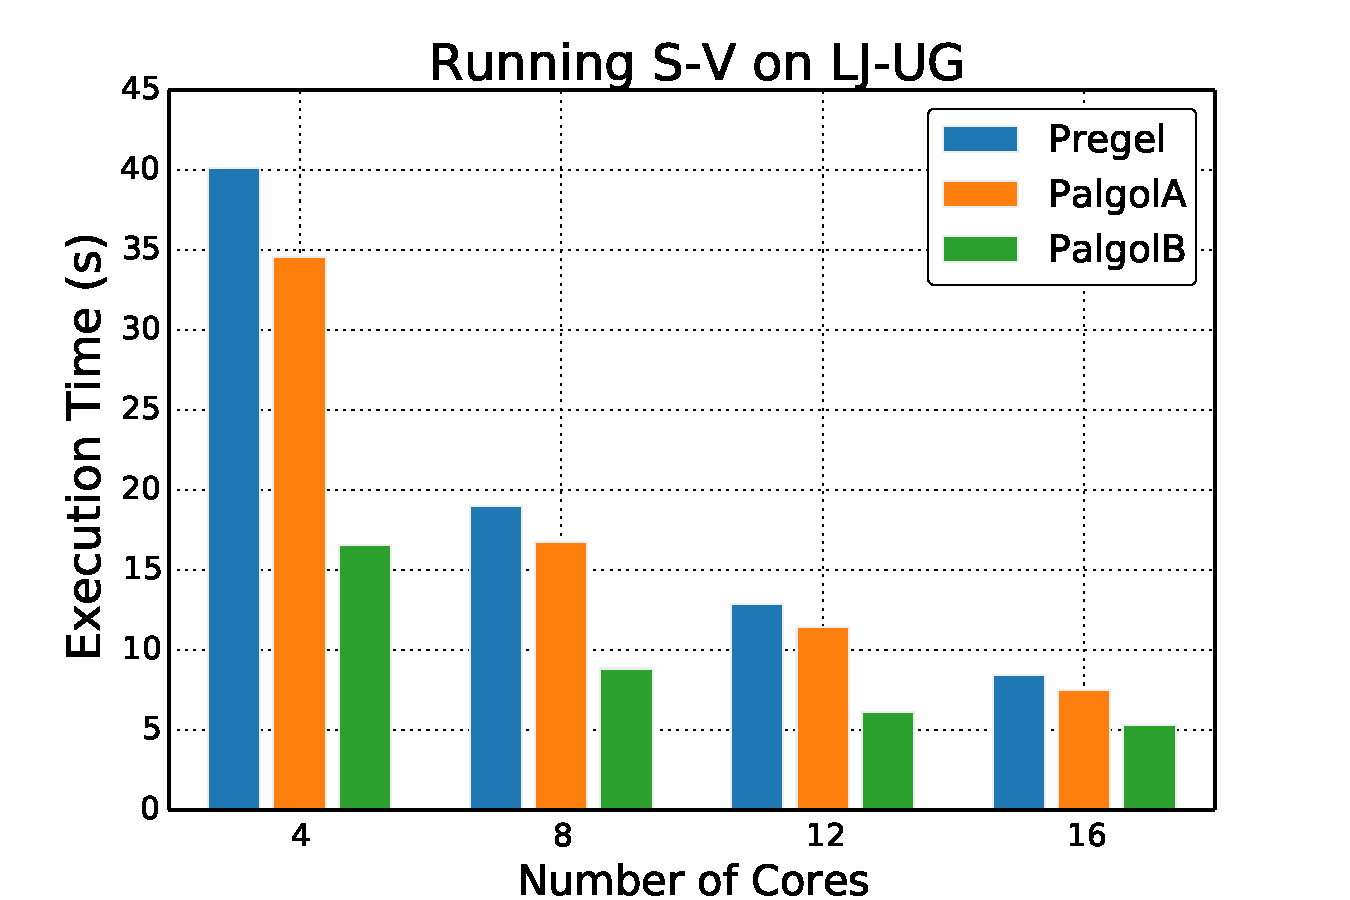
\includegraphics[width=0.48\textwidth]{plot/exec_svppa_LJ-UG.pdf}
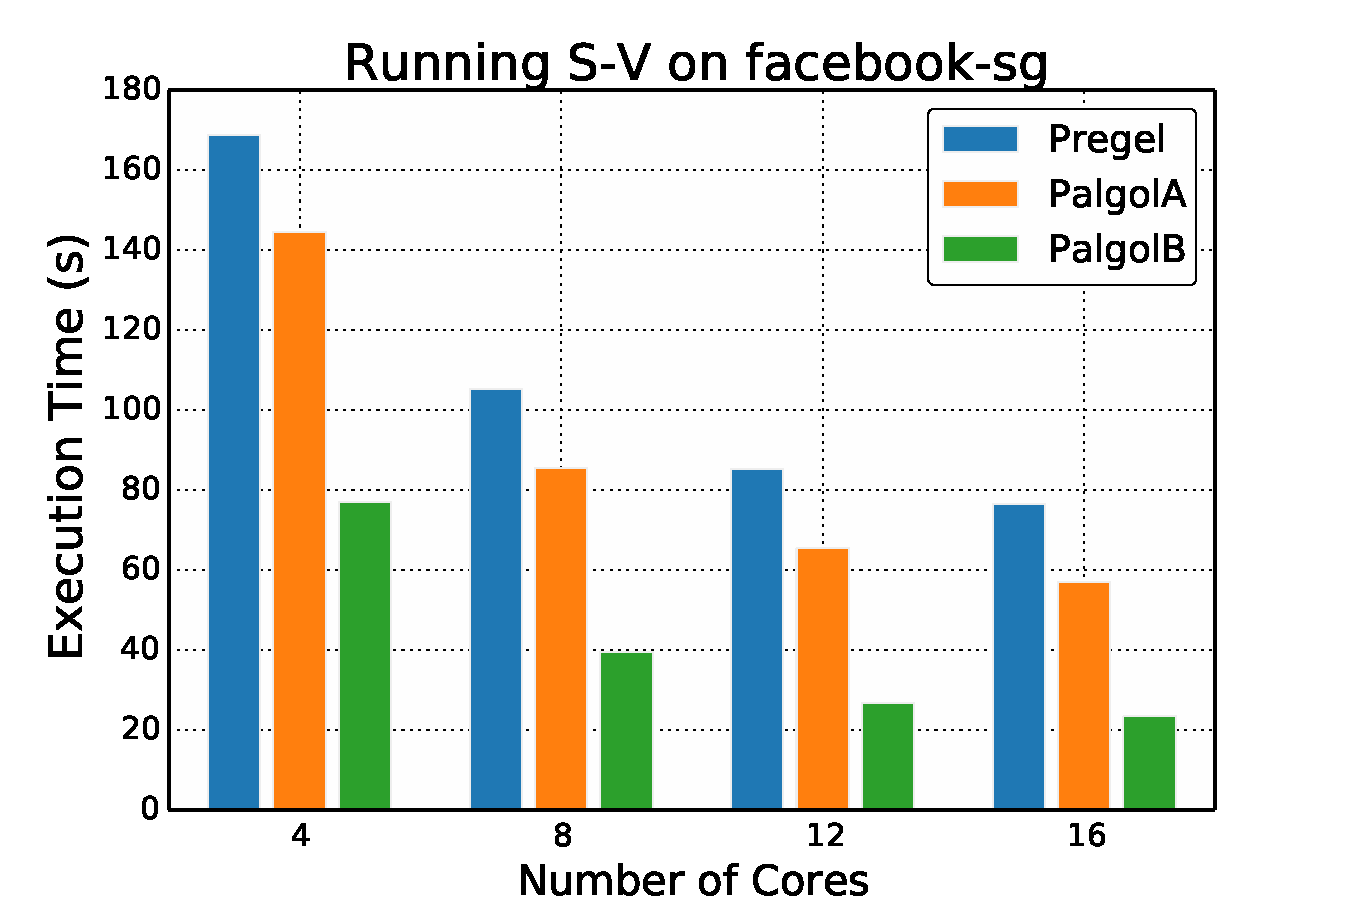
\includegraphics[width=0.48\textwidth]{plot/exec_svppa_facebook-sg.pdf}
\caption{Comparison of the execution time. PalgolA is the compiler-generated program on Pregel+, and PalgolB is the hand-transformed program on our custom Pregel system.}
\label{fig:exec}
\end{comment}

\chapter{Related Work}

Google's Pregel \cite{pregel} proposed the vertex-centric computing paradigm, which allows programmers to think naturally like a vertex when designing distributed graph algorithms.
Some graph-centric (or block-centric) systems like Giraph\plus\cite{thinkgraph}, GoFFish~\cite{goffish} and Blogel~\cite{blogel} extend Pregel's vertex-centric approach by making the partitioning mechanism open to programmers, but it is still unclear how to optimize general vertex-centric algorithms (especially those complicated ones containing non-trivial communication patterns) using such extension.

Domain-Specific Languages (DSLs) are a well-known mechanism for describing solutions in specialized domains.
To ease Pregel programming, many DSLs have been proposed, such as Palovca~\cite{palovca}, s6raph~\cite{s6raph}, Fregel~\cite{fregel} and Green-Marl~\cite{green14}.
We briefly introduce each of them below.

Palovca~\cite{palovca} exposes the Pregel APIs in Haskell using a monad, and a vertex-centric program is written in a low-level way like in typical Pregel systems.
Since this language is still low-level, programmers are faced with the same challenges in Pregel programming, mainly having to tackle all low-level details.

At the other extreme, the s6raph system~\cite{s6raph} is a special graph processing framework with a functional interface.
It models a particular type of iterative vertex-centric computation by six programmer-specified functions, and can only express graph algorithms that contain a single iterative computation (such as PageRank and Shortest Path), whereas many practical Pregel algorithms are far more complicated.
%In exchange, s6raph programs can be written concisely.

A more comparable and (in fact) closely related piece of work is Fregel~\cite{fregel}, which is a functional DSL for declarative programming on big graphs.
In Fregel, a vertex-centric computation is represented by a pure step function that takes a graph as input and produces a new vertex state;
such functions can then be composed using a set of predefined higher-order functions to implement a complete graph algorithm.
Palgol borrows this idea in the language design by letting programmers write atomic vertex-centric computations called Palgol steps, and put them together using two combinators, namely sequence and iteration.
%The combinators we choose can be naturally optimized by the fusion optimization (borrowing the idea of ``intra-loop state merging'' in Green-Marl)
%Nevertheless, the choices of the combinators are not the same.
%It prevents programmers from writing invalid programs and helps people to better understand the behavior of a vertex-centric program.
%A Palgol step is more expressive than a step function, due to the following two reasons:
Compared with Fregel, the main strength of Palgol is in its remote access capabilities:
\begin{itemize}
 \item a Palgol step consists of local computation and remote updating phases, whereas a Fregel step function can be thought of as only describing local computation, lacking the ability to modify other vertices' states;
 \item even when considering local computation only, Palgol has highly declarative \textit{field access expressions} to express remote reading of arbitrary vertices, whereas Fregel allows only neighboring access.
\end{itemize}
These two features are however essential for implementing the examples in \autoref{sec:taste}, especially the S-V algorithm.
Moreover, when implementing the same graph algorithm, the execution time of Fregel is around an order of magnitude slower than human written code.
Palgol shows that Fregel's combinator-based design can benefit from Green-Marl's fusion optimizations~(\autoref{sec:trans-iter}) and achieve efficiency comparable to hand-written code.

Another comparable DSL is Green-Marl~\cite{green12}, which lets programmers describe graph algorithms in a higher-level imperative language.
This language is initially proposed for graph processing on the shared-memory model, and a ``Pregel-canonical'' subset of its programs can be compiled to Pregel.
Since it does not have a Pregel-specific language design, programmers may easily get compilation errors if they are not familiar with the implementation of the compiler.
In contrast, Palgol (and Fregel) programs are by construction vertex-centric and distinguish the current and previous states for the vertices, and thus have a closer correspondence with the Pregel model.
For remote reads, Green-Marl only supports neighboring access, so it suffers the same problem as Fregel where programmers cannot fetch data from an arbitrary vertex.
While it supports graph traversal skeletons like BFS and DFS, these traversals can be encoded as neighborhood access with modest effort, so it actually has the same expressiveness as Fregel in terms of remote reading.
Green-Marl supports remote writing, but according to our experience, it is quite restricted, and at least cannot be used inside a loop iterating over a neighbor list, and thus is less expressive than Palgol.

\chapter{Conclusion}
\label{sec:conclusions}

This work introduced Palgol, a high-level domain-specific language for Pregel systems with flexible remote data access, which makes it possible for programmers to express Pregel algorithms that communicate over dynamic internal data structures.
We have demonstrated the power of Palgol's remote access by giving two representative examples, the S-V algorithm and the list ranking algorithm, and presented the key algorithm for compiling remote access.
Moreover, we have shown that Fregel's more structured approach to vertex-centric computing, our compilation algorithm for remote access and Green-Marl's optimization techniques can work together perfectly, and the experiment results show that graph algorithms written in Palgol can be compiled to efficient Pregel programs comparable to human written ones.

We expect Palgol's remote access capabilities to help with developing more sophisticated vertex-centric algorithms where each vertex decides its action by looking at not only its immediate neighborhood but also an extended and dynamic neighborhood.
The S-V and list ranking algorithms are just a start --- for a differently flavored example, graph pattern matching~\cite{graphpm} might be greatly simplified when the pattern has a constant size and can be translated declaratively as a remote access expression deciding whether a vertex and some other ``nearby'' vertices exhibit the pattern.
Algorithm design and language design are interdependent, with algorithmic ideas prompting more language features and higher-level languages making it easier to formulate and reason about more sophisticated algorithms.
We believe that Palgol is a much-needed advance in language design that can bring vertex-centric algorithm design forward.

As for future work, we will compile Palgol to our custom Pregel system, making these two pieces of works a intuitive and efficient solution for vertex-centric graph processing.

% =====================================================
%  Back Matter
% =====================================================

%\backmatter


% =====================================================
%  Bibliography
% =====================================================

%\bibliographystyle{plain}
\bibliographystyle{unsrt}
\bibliography{ref}


% =====================================================
%  Appendices
% =====================================================

\begin{appendices}

%\include{Manuscript/Tips/tips}

\end{appendices}


\end{document}
